% Options for packages loaded elsewhere
% Options for packages loaded elsewhere
\PassOptionsToPackage{unicode}{hyperref}
\PassOptionsToPackage{hyphens}{url}
\PassOptionsToPackage{dvipsnames,svgnames,x11names}{xcolor}
%
\documentclass[
  letterpaper,
  oneside,
  11pt]{article}
\usepackage{xcolor}
\usepackage[left=1in,right=1in,top=1in,bottom=1in]{geometry}
\usepackage{amsmath,amssymb}
\setcounter{secnumdepth}{-\maxdimen} % remove section numbering
\usepackage{iftex}
\ifPDFTeX
  \usepackage[T1]{fontenc}
  \usepackage[utf8]{inputenc}
  \usepackage{textcomp} % provide euro and other symbols
\else % if luatex or xetex
  \usepackage{unicode-math} % this also loads fontspec
  \defaultfontfeatures{Scale=MatchLowercase}
  \defaultfontfeatures[\rmfamily]{Ligatures=TeX,Scale=1}
\fi
\usepackage{lmodern}
\ifPDFTeX\else
  % xetex/luatex font selection
\fi
% Use upquote if available, for straight quotes in verbatim environments
\IfFileExists{upquote.sty}{\usepackage{upquote}}{}
\IfFileExists{microtype.sty}{% use microtype if available
  \usepackage[]{microtype}
  \UseMicrotypeSet[protrusion]{basicmath} % disable protrusion for tt fonts
}{}
\makeatletter
\@ifundefined{KOMAClassName}{% if non-KOMA class
  \IfFileExists{parskip.sty}{%
    \usepackage{parskip}
  }{% else
    \setlength{\parindent}{0pt}
    \setlength{\parskip}{6pt plus 2pt minus 1pt}}
}{% if KOMA class
  \KOMAoptions{parskip=half}}
\makeatother
% Make \paragraph and \subparagraph free-standing
\makeatletter
\ifx\paragraph\undefined\else
  \let\oldparagraph\paragraph
  \renewcommand{\paragraph}{
    \@ifstar
      \xxxParagraphStar
      \xxxParagraphNoStar
  }
  \newcommand{\xxxParagraphStar}[1]{\oldparagraph*{#1}\mbox{}}
  \newcommand{\xxxParagraphNoStar}[1]{\oldparagraph{#1}\mbox{}}
\fi
\ifx\subparagraph\undefined\else
  \let\oldsubparagraph\subparagraph
  \renewcommand{\subparagraph}{
    \@ifstar
      \xxxSubParagraphStar
      \xxxSubParagraphNoStar
  }
  \newcommand{\xxxSubParagraphStar}[1]{\oldsubparagraph*{#1}\mbox{}}
  \newcommand{\xxxSubParagraphNoStar}[1]{\oldsubparagraph{#1}\mbox{}}
\fi
\makeatother

\usepackage{color}
\usepackage{fancyvrb}
\newcommand{\VerbBar}{|}
\newcommand{\VERB}{\Verb[commandchars=\\\{\}]}
\DefineVerbatimEnvironment{Highlighting}{Verbatim}{commandchars=\\\{\}}
% Add ',fontsize=\small' for more characters per line
\usepackage{framed}
\definecolor{shadecolor}{RGB}{241,243,245}
\newenvironment{Shaded}{\begin{snugshade}}{\end{snugshade}}
\newcommand{\AlertTok}[1]{\textcolor[rgb]{0.68,0.00,0.00}{#1}}
\newcommand{\AnnotationTok}[1]{\textcolor[rgb]{0.37,0.37,0.37}{#1}}
\newcommand{\AttributeTok}[1]{\textcolor[rgb]{0.40,0.45,0.13}{#1}}
\newcommand{\BaseNTok}[1]{\textcolor[rgb]{0.68,0.00,0.00}{#1}}
\newcommand{\BuiltInTok}[1]{\textcolor[rgb]{0.00,0.23,0.31}{#1}}
\newcommand{\CharTok}[1]{\textcolor[rgb]{0.13,0.47,0.30}{#1}}
\newcommand{\CommentTok}[1]{\textcolor[rgb]{0.37,0.37,0.37}{#1}}
\newcommand{\CommentVarTok}[1]{\textcolor[rgb]{0.37,0.37,0.37}{\textit{#1}}}
\newcommand{\ConstantTok}[1]{\textcolor[rgb]{0.56,0.35,0.01}{#1}}
\newcommand{\ControlFlowTok}[1]{\textcolor[rgb]{0.00,0.23,0.31}{\textbf{#1}}}
\newcommand{\DataTypeTok}[1]{\textcolor[rgb]{0.68,0.00,0.00}{#1}}
\newcommand{\DecValTok}[1]{\textcolor[rgb]{0.68,0.00,0.00}{#1}}
\newcommand{\DocumentationTok}[1]{\textcolor[rgb]{0.37,0.37,0.37}{\textit{#1}}}
\newcommand{\ErrorTok}[1]{\textcolor[rgb]{0.68,0.00,0.00}{#1}}
\newcommand{\ExtensionTok}[1]{\textcolor[rgb]{0.00,0.23,0.31}{#1}}
\newcommand{\FloatTok}[1]{\textcolor[rgb]{0.68,0.00,0.00}{#1}}
\newcommand{\FunctionTok}[1]{\textcolor[rgb]{0.28,0.35,0.67}{#1}}
\newcommand{\ImportTok}[1]{\textcolor[rgb]{0.00,0.46,0.62}{#1}}
\newcommand{\InformationTok}[1]{\textcolor[rgb]{0.37,0.37,0.37}{#1}}
\newcommand{\KeywordTok}[1]{\textcolor[rgb]{0.00,0.23,0.31}{\textbf{#1}}}
\newcommand{\NormalTok}[1]{\textcolor[rgb]{0.00,0.23,0.31}{#1}}
\newcommand{\OperatorTok}[1]{\textcolor[rgb]{0.37,0.37,0.37}{#1}}
\newcommand{\OtherTok}[1]{\textcolor[rgb]{0.00,0.23,0.31}{#1}}
\newcommand{\PreprocessorTok}[1]{\textcolor[rgb]{0.68,0.00,0.00}{#1}}
\newcommand{\RegionMarkerTok}[1]{\textcolor[rgb]{0.00,0.23,0.31}{#1}}
\newcommand{\SpecialCharTok}[1]{\textcolor[rgb]{0.37,0.37,0.37}{#1}}
\newcommand{\SpecialStringTok}[1]{\textcolor[rgb]{0.13,0.47,0.30}{#1}}
\newcommand{\StringTok}[1]{\textcolor[rgb]{0.13,0.47,0.30}{#1}}
\newcommand{\VariableTok}[1]{\textcolor[rgb]{0.07,0.07,0.07}{#1}}
\newcommand{\VerbatimStringTok}[1]{\textcolor[rgb]{0.13,0.47,0.30}{#1}}
\newcommand{\WarningTok}[1]{\textcolor[rgb]{0.37,0.37,0.37}{\textit{#1}}}

\usepackage{longtable,booktabs,array}
\newcounter{none} % for unnumbered tables
\usepackage{calc} % for calculating minipage widths
% Correct order of tables after \paragraph or \subparagraph
\usepackage{etoolbox}
\makeatletter
\patchcmd\longtable{\par}{\if@noskipsec\mbox{}\fi\par}{}{}
\makeatother
% Allow footnotes in longtable head/foot
\IfFileExists{footnotehyper.sty}{\usepackage{footnotehyper}}{\usepackage{footnote}}
\makesavenoteenv{longtable}
\usepackage{graphicx}
\makeatletter
\newsavebox\pandoc@box
\newcommand*\pandocbounded[1]{% scales image to fit in text height/width
  \sbox\pandoc@box{#1}%
  \Gscale@div\@tempa{\textheight}{\dimexpr\ht\pandoc@box+\dp\pandoc@box\relax}%
  \Gscale@div\@tempb{\linewidth}{\wd\pandoc@box}%
  \ifdim\@tempb\p@<\@tempa\p@\let\@tempa\@tempb\fi% select the smaller of both
  \ifdim\@tempa\p@<\p@\scalebox{\@tempa}{\usebox\pandoc@box}%
  \else\usebox{\pandoc@box}%
  \fi%
}
% Set default figure placement to htbp
\def\fps@figure{htbp}
\makeatother





\setlength{\emergencystretch}{3em} % prevent overfull lines

\providecommand{\tightlist}{%
  \setlength{\itemsep}{0pt}\setlength{\parskip}{0pt}}



 


\usepackage[utf8]{inputenc}
\usepackage{graphicx}
\usepackage{float}
\makeatletter
\@ifpackageloaded{caption}{}{\usepackage{caption}}
\AtBeginDocument{%
\ifdefined\contentsname
  \renewcommand*\contentsname{Table of contents}
\else
  \newcommand\contentsname{Table of contents}
\fi
\ifdefined\listfigurename
  \renewcommand*\listfigurename{List of Figures}
\else
  \newcommand\listfigurename{List of Figures}
\fi
\ifdefined\listtablename
  \renewcommand*\listtablename{List of Tables}
\else
  \newcommand\listtablename{List of Tables}
\fi
\ifdefined\figurename
  \renewcommand*\figurename{Figure}
\else
  \newcommand\figurename{Figure}
\fi
\ifdefined\tablename
  \renewcommand*\tablename{Table}
\else
  \newcommand\tablename{Table}
\fi
}
\@ifpackageloaded{float}{}{\usepackage{float}}
\floatstyle{ruled}
\@ifundefined{c@chapter}{\newfloat{codelisting}{h}{lop}}{\newfloat{codelisting}{h}{lop}[chapter]}
\floatname{codelisting}{Listing}
\newcommand*\listoflistings{\listof{codelisting}{List of Listings}}
\makeatother
\makeatletter
\makeatother
\makeatletter
\@ifpackageloaded{caption}{}{\usepackage{caption}}
\@ifpackageloaded{subcaption}{}{\usepackage{subcaption}}
\makeatother
\usepackage{bookmark}
\IfFileExists{xurl.sty}{\usepackage{xurl}}{} % add URL line breaks if available
\urlstyle{same}
\hypersetup{
  pdftitle={Market Intelligence - Club Profitability Analysis},
  pdfauthor={jortega},
  colorlinks=true,
  linkcolor={blue},
  filecolor={Maroon},
  citecolor={Blue},
  urlcolor={Blue},
  pdfcreator={LaTeX via pandoc}}


\title{Market Intelligence - Club Profitability Analysis}
\author{jortega}
\date{2026-08-01}
\begin{document}
\maketitle


\begin{Shaded}
\begin{Highlighting}[]
\CommentTok{\# Read data from the project root\textquotesingle{}s data directory}
\NormalTok{club\_master }\OtherTok{\textless{}{-}} \FunctionTok{readRDS}\NormalTok{(}\StringTok{"data/club\_master.rds"}\NormalTok{)}
\NormalTok{members\_year }\OtherTok{\textless{}{-}} \FunctionTok{readRDS}\NormalTok{(}\StringTok{"data/members\_year.rds"}\NormalTok{)}
\NormalTok{club\_performance }\OtherTok{\textless{}{-}} \FunctionTok{readRDS}\NormalTok{(}\StringTok{"data/club\_performance.rds"}\NormalTok{)}
\NormalTok{club\_perf\_year4 }\OtherTok{\textless{}{-}} \FunctionTok{readRDS}\NormalTok{(}\StringTok{"data/club\_perf\_year4.rds"}\NormalTok{)}
\NormalTok{rf\_importance }\OtherTok{\textless{}{-}} \FunctionTok{readRDS}\NormalTok{(}\StringTok{"data/rf\_importance.rds"}\NormalTok{)}
\end{Highlighting}
\end{Shaded}

\section{Report}\label{report}

\section{Title: Market Intelligence}\label{title-market-intelligence}

\section{Subtitle: Club characteristics and Market Factors Driving
Profitability}\label{subtitle-club-characteristics-and-market-factors-driving-profitability}

\begin{Shaded}
\begin{Highlighting}[]
\CommentTok{\# Custom color palette (including chocolate3)}
\NormalTok{custom\_palette }\OtherTok{\textless{}{-}} \FunctionTok{c}\NormalTok{(}
  \StringTok{"chocolate3"}\NormalTok{,    }\CommentTok{\# Your requested color}
  \StringTok{"\#E69F00"}\NormalTok{,       }\CommentTok{\# Orange}
  \StringTok{"\#56B4E9"}\NormalTok{,       }\CommentTok{\# Sky Blue}
  \StringTok{"\#009E73"}\NormalTok{,       }\CommentTok{\# Teal}
  \StringTok{"\#F0E442"}        \CommentTok{\# Yellow}
\NormalTok{)}

\CommentTok{\# Define a reusable theme}
\NormalTok{fit\_theme }\OtherTok{\textless{}{-}} \ControlFlowTok{function}\NormalTok{() \{}
  \FunctionTok{theme\_minimal}\NormalTok{() }\SpecialCharTok{+}
    \FunctionTok{theme}\NormalTok{(}
      \AttributeTok{legend.position =} \StringTok{"none"}\NormalTok{,}
      \AttributeTok{plot.title =} \FunctionTok{element\_text}\NormalTok{(}\AttributeTok{face =} \StringTok{"bold"}\NormalTok{, }\AttributeTok{size =} \DecValTok{14}\NormalTok{, }\AttributeTok{hjust =} \FloatTok{0.5}\NormalTok{, }\AttributeTok{color =} \StringTok{"gray30"}\NormalTok{),}
      \AttributeTok{plot.subtitle =} \FunctionTok{element\_text}\NormalTok{(}\AttributeTok{face =} \StringTok{"italic"}\NormalTok{, }\AttributeTok{size =} \DecValTok{10}\NormalTok{, }\AttributeTok{hjust =} \FloatTok{0.5}\NormalTok{, }\AttributeTok{color =} \StringTok{"gray30"}\NormalTok{),}
      \AttributeTok{axis.title =} \FunctionTok{element\_text}\NormalTok{(}\AttributeTok{face =} \StringTok{"bold"}\NormalTok{, }\AttributeTok{size =} \DecValTok{12}\NormalTok{, }\AttributeTok{color =} \StringTok{"gray30"}\NormalTok{),}
      \AttributeTok{axis.text =} \FunctionTok{element\_text}\NormalTok{(}\AttributeTok{size =} \DecValTok{11}\NormalTok{, }\AttributeTok{color =} \StringTok{"gray30"}\NormalTok{, }\AttributeTok{family =} \StringTok{"Helvetica"}\NormalTok{),}
      \AttributeTok{strip.text =} \FunctionTok{element\_text}\NormalTok{(}\AttributeTok{face =} \StringTok{"bold"}\NormalTok{, }\AttributeTok{size =} \DecValTok{10}\NormalTok{, }\AttributeTok{color =} \StringTok{"gray30"}\NormalTok{),}
      \AttributeTok{panel.grid.minor =} \FunctionTok{element\_blank}\NormalTok{(),}
      \AttributeTok{panel.grid.major =} \FunctionTok{element\_blank}\NormalTok{()}
\NormalTok{    )}
\NormalTok{\}}
\end{Highlighting}
\end{Shaded}

\subsection{Histograms - Active Members, Revenue Per SqFt, EBITDA Per
SqFt}\label{histograms---active-members-revenue-per-sqft-ebitda-per-sqft}

\emph{Chart: Distribution of Active Members, EBITDA and Revenue}

\emph{Text: The average mature club has 8,000 active members, with
revenue close to \$100 (per sqft) and profit of \$40 (per sqft).}

\begin{Shaded}
\begin{Highlighting}[]
\CommentTok{\# Prepare Data}
\NormalTok{perf\_metrics }\OtherTok{\textless{}{-}}\NormalTok{ club\_perf\_year4 }\SpecialCharTok{\%\textgreater{}\%}
  \FunctionTok{select}\NormalTok{(RevenuePerSqFt, EBITDAPerSqFt, ActiveMembers) }\SpecialCharTok{\%\textgreater{}\%}
  \FunctionTok{pivot\_longer}\NormalTok{(}\AttributeTok{cols =} \FunctionTok{everything}\NormalTok{(), }\AttributeTok{names\_to =} \StringTok{"PerformanceMetric"}\NormalTok{, }\AttributeTok{values\_to =} \StringTok{"Value"}\NormalTok{)}

\CommentTok{\# Calculate median values for each PerformanceMetric}
\NormalTok{median\_values }\OtherTok{\textless{}{-}}\NormalTok{ perf\_metrics }\SpecialCharTok{\%\textgreater{}\%}
  \FunctionTok{group\_by}\NormalTok{(PerformanceMetric) }\SpecialCharTok{\%\textgreater{}\%}
  \FunctionTok{summarise}\NormalTok{(}\AttributeTok{Median =} \FunctionTok{median}\NormalTok{(Value, }\AttributeTok{na.rm =} \ConstantTok{TRUE}\NormalTok{)) }\SpecialCharTok{\%\textgreater{}\%}
  \FunctionTok{ungroup}\NormalTok{()}

\CommentTok{\# Plot with vertical faceting and custom colors}
\FunctionTok{ggplot}\NormalTok{(perf\_metrics, }\FunctionTok{aes}\NormalTok{(}\AttributeTok{x =}\NormalTok{ Value, }\AttributeTok{fill =}\NormalTok{ PerformanceMetric)) }\SpecialCharTok{+}
  \FunctionTok{geom\_histogram}\NormalTok{(}\AttributeTok{bins =} \DecValTok{10}\NormalTok{, }\AttributeTok{alpha =} \FloatTok{0.7}\NormalTok{, }\AttributeTok{position =} \StringTok{"dodge"}\NormalTok{) }\SpecialCharTok{+}
  \FunctionTok{geom\_vline}\NormalTok{(}
    \AttributeTok{data =}\NormalTok{ median\_values,}
    \FunctionTok{aes}\NormalTok{(}\AttributeTok{xintercept =}\NormalTok{ Median),}
    \AttributeTok{linetype =} \StringTok{"dotted"}\NormalTok{,}
    \AttributeTok{color =} \StringTok{"indianred4"}\NormalTok{,}
    \AttributeTok{linewidth =} \FloatTok{0.8}
\NormalTok{  ) }\SpecialCharTok{+}
  \FunctionTok{scale\_fill\_manual}\NormalTok{(}\AttributeTok{values =}\NormalTok{ custom\_palette) }\SpecialCharTok{+}  \CommentTok{\# Apply custom palette}
  \FunctionTok{facet\_wrap}\NormalTok{(}\SpecialCharTok{\textasciitilde{}}\NormalTok{ PerformanceMetric, }\AttributeTok{scales =} \StringTok{"free\_x"}\NormalTok{) }\SpecialCharTok{+}  \CommentTok{\# Vertical faceting}
  \FunctionTok{labs}\NormalTok{(}
    \AttributeTok{title =} \StringTok{"Distribution of Performance Metrics"}\NormalTok{,}
    \AttributeTok{subtitle =} \StringTok{"Mature Clubs. Vertical dotted lines indicate median values"}\NormalTok{,}
    \AttributeTok{x =} \StringTok{""}\NormalTok{,}
    \AttributeTok{y =} \StringTok{"Frequency"}
\NormalTok{  ) }\SpecialCharTok{+}
  \FunctionTok{fit\_theme}\NormalTok{()}
\end{Highlighting}
\end{Shaded}

\pandocbounded{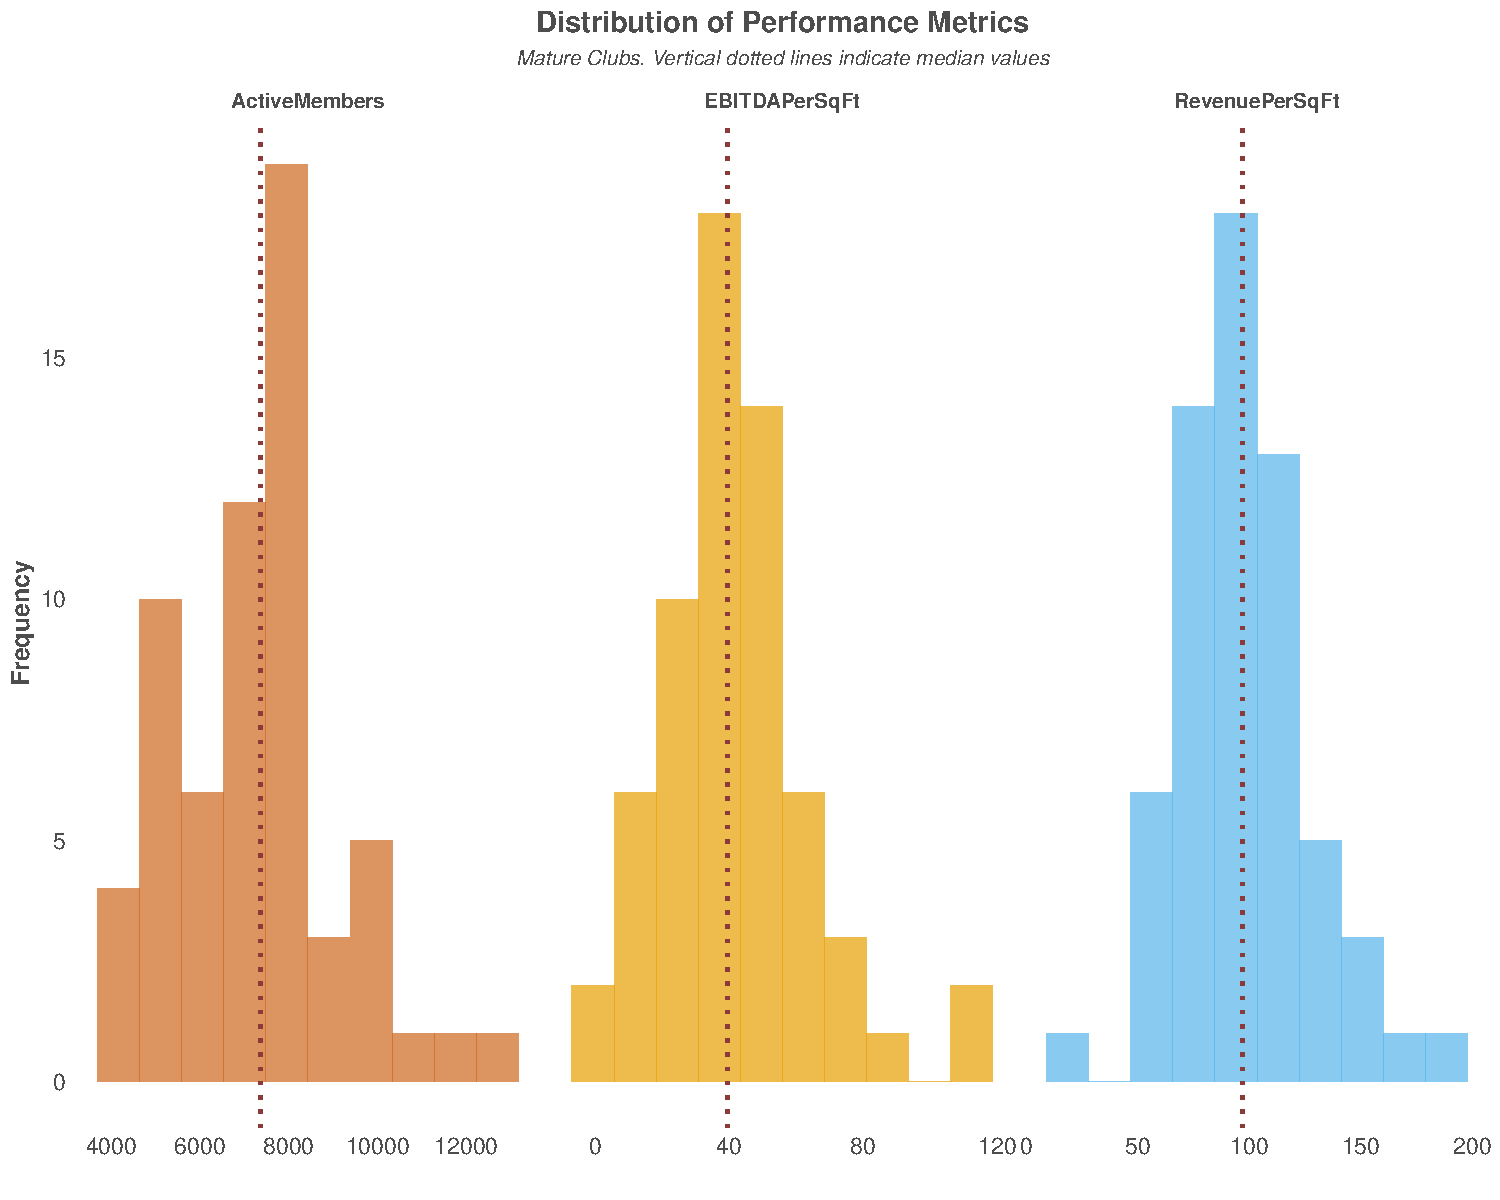
\includegraphics[keepaspectratio]{fit_report_profit_files/figure-pdf/histograms-1.pdf}}

\subsection{Scatter Plot: Revenue Per SqFt vs EBITDA Per
SqFt}\label{scatter-plot-revenue-per-sqft-vs-ebitda-per-sqft}

\emph{Chart: Relationship between Revenue and Profitability}

\emph{Text: Not surprisingly higher revenue leads to higher profits;
there are three clubs that stand out: Catonsville, Penn Station and
Golden Ring.}

\begin{Shaded}
\begin{Highlighting}[]
\CommentTok{\# Scatterplot of RevenuePerSqFt vs. EBITDAPerSqFt with fitted line}
\FunctionTok{ggplot}\NormalTok{(club\_perf\_year4, }\FunctionTok{aes}\NormalTok{(}\AttributeTok{x =}\NormalTok{ RevenuePerSqFt, }\AttributeTok{y =}\NormalTok{ EBITDAPerSqFt)) }\SpecialCharTok{+}
  \FunctionTok{geom\_point}\NormalTok{(}
    \FunctionTok{aes}\NormalTok{(}\AttributeTok{color =}\NormalTok{ EBITDAPerSqFt }\SpecialCharTok{\textgreater{}} \DecValTok{80}\NormalTok{),}
    \AttributeTok{alpha =} \FloatTok{0.6}\NormalTok{,}
    \AttributeTok{size =} \DecValTok{4}
\NormalTok{  ) }\SpecialCharTok{+}
  \FunctionTok{scale\_color\_manual}\NormalTok{(}
    \AttributeTok{values =} \FunctionTok{c}\NormalTok{(}\StringTok{"FALSE"} \OtherTok{=}\NormalTok{ custom\_palette[}\DecValTok{1}\NormalTok{], }\StringTok{"TRUE"} \OtherTok{=}\NormalTok{ custom\_palette[}\DecValTok{4}\NormalTok{]),}
\NormalTok{  ) }\SpecialCharTok{+}
  \FunctionTok{geom\_text}\NormalTok{(}
    \AttributeTok{data =}\NormalTok{ club\_perf\_year4 }\SpecialCharTok{\%\textgreater{}\%} \FunctionTok{filter}\NormalTok{(EBITDAPerSqFt }\SpecialCharTok{\textgreater{}} \DecValTok{80}\NormalTok{),}
    \FunctionTok{aes}\NormalTok{(}\AttributeTok{x =}\NormalTok{ RevenuePerSqFt, }\AttributeTok{y =}\NormalTok{ EBITDAPerSqFt, }\AttributeTok{label =}\NormalTok{ ClubName),}
    \AttributeTok{hjust =} \FloatTok{1.2}\NormalTok{,}
    \AttributeTok{vjust =} \DecValTok{0}\NormalTok{,}
    \AttributeTok{color =}\NormalTok{ custom\_palette[}\DecValTok{4}\NormalTok{],}
    \AttributeTok{size =} \FloatTok{3.5}\NormalTok{,}
    \AttributeTok{fontface =} \StringTok{"bold"}
\NormalTok{  ) }\SpecialCharTok{+}
  \FunctionTok{geom\_text}\NormalTok{(}
    \AttributeTok{data =}\NormalTok{ club\_perf\_year4 }\SpecialCharTok{\%\textgreater{}\%} \FunctionTok{filter}\NormalTok{(RevenuePerSqFt }\SpecialCharTok{\textless{}} \DecValTok{40}\NormalTok{),}
    \FunctionTok{aes}\NormalTok{(}\AttributeTok{x =}\NormalTok{ RevenuePerSqFt, }\AttributeTok{y =}\NormalTok{ EBITDAPerSqFt, }\AttributeTok{label =}\NormalTok{ ClubName),}
    \AttributeTok{hjust =} \FloatTok{0.1}\NormalTok{,}
    \AttributeTok{vjust =} \SpecialCharTok{{-}}\DecValTok{1}\NormalTok{,}
    \AttributeTok{color =}\NormalTok{ custom\_palette[}\DecValTok{1}\NormalTok{],}
    \AttributeTok{size =} \FloatTok{3.5}\NormalTok{,}
    \AttributeTok{fontface =} \StringTok{"bold"}
\NormalTok{  ) }\SpecialCharTok{+}
  \FunctionTok{geom\_hline}\NormalTok{(}
    \AttributeTok{yintercept =} \DecValTok{0}\NormalTok{,  }\CommentTok{\# Horizontal line at EBITDAPerSqFt == 0}
    \AttributeTok{color =}\NormalTok{ custom\_palette[}\DecValTok{2}\NormalTok{],}
    \AttributeTok{linetype =} \StringTok{"solid"}\NormalTok{,}
    \AttributeTok{linewidth =} \FloatTok{0.5}
\NormalTok{  ) }\SpecialCharTok{+}
  \FunctionTok{geom\_smooth}\NormalTok{(}
    \AttributeTok{method =} \StringTok{"lm"}\NormalTok{,  }\CommentTok{\# Linear regression}
    \AttributeTok{se =} \ConstantTok{FALSE}\NormalTok{,}
    \AttributeTok{color =}\NormalTok{ custom\_palette[}\DecValTok{3}\NormalTok{],}
    \AttributeTok{linewidth =} \FloatTok{0.8}\NormalTok{,}
    \AttributeTok{linetype =} \StringTok{"dashed"}
\NormalTok{  ) }\SpecialCharTok{+}
  \FunctionTok{scale\_y\_continuous}\NormalTok{(}\AttributeTok{breaks =} \FunctionTok{seq}\NormalTok{(}\SpecialCharTok{{-}}\DecValTok{20}\NormalTok{, }\DecValTok{140}\NormalTok{, }\AttributeTok{by =} \DecValTok{20}\NormalTok{)) }\SpecialCharTok{+}
  \FunctionTok{labs}\NormalTok{(}
    \AttributeTok{title =} \StringTok{"Revenue vs. Profitability"}\NormalTok{,}
    \AttributeTok{subtitle =} \StringTok{"Clubs with EBITDA Per SqFt \textgreater{} 80 are highlighted"}\NormalTok{,}
    \AttributeTok{x =} \StringTok{"Revenue Per SqFt ($)"}\NormalTok{,}
    \AttributeTok{y =} \StringTok{"EBITDA Per SqFt ($)"}
\NormalTok{  ) }\SpecialCharTok{+}
  \FunctionTok{fit\_theme}\NormalTok{() }\SpecialCharTok{+}
  \FunctionTok{theme}\NormalTok{(}
    \AttributeTok{panel.grid.major.y =} \FunctionTok{element\_line}\NormalTok{(}\AttributeTok{color =} \StringTok{"gray90"}\NormalTok{, }\AttributeTok{linewidth =} \FloatTok{0.2}\NormalTok{)}
\NormalTok{  )}
\end{Highlighting}
\end{Shaded}

\begin{verbatim}
`geom_smooth()` using formula = 'y ~ x'
\end{verbatim}

\pandocbounded{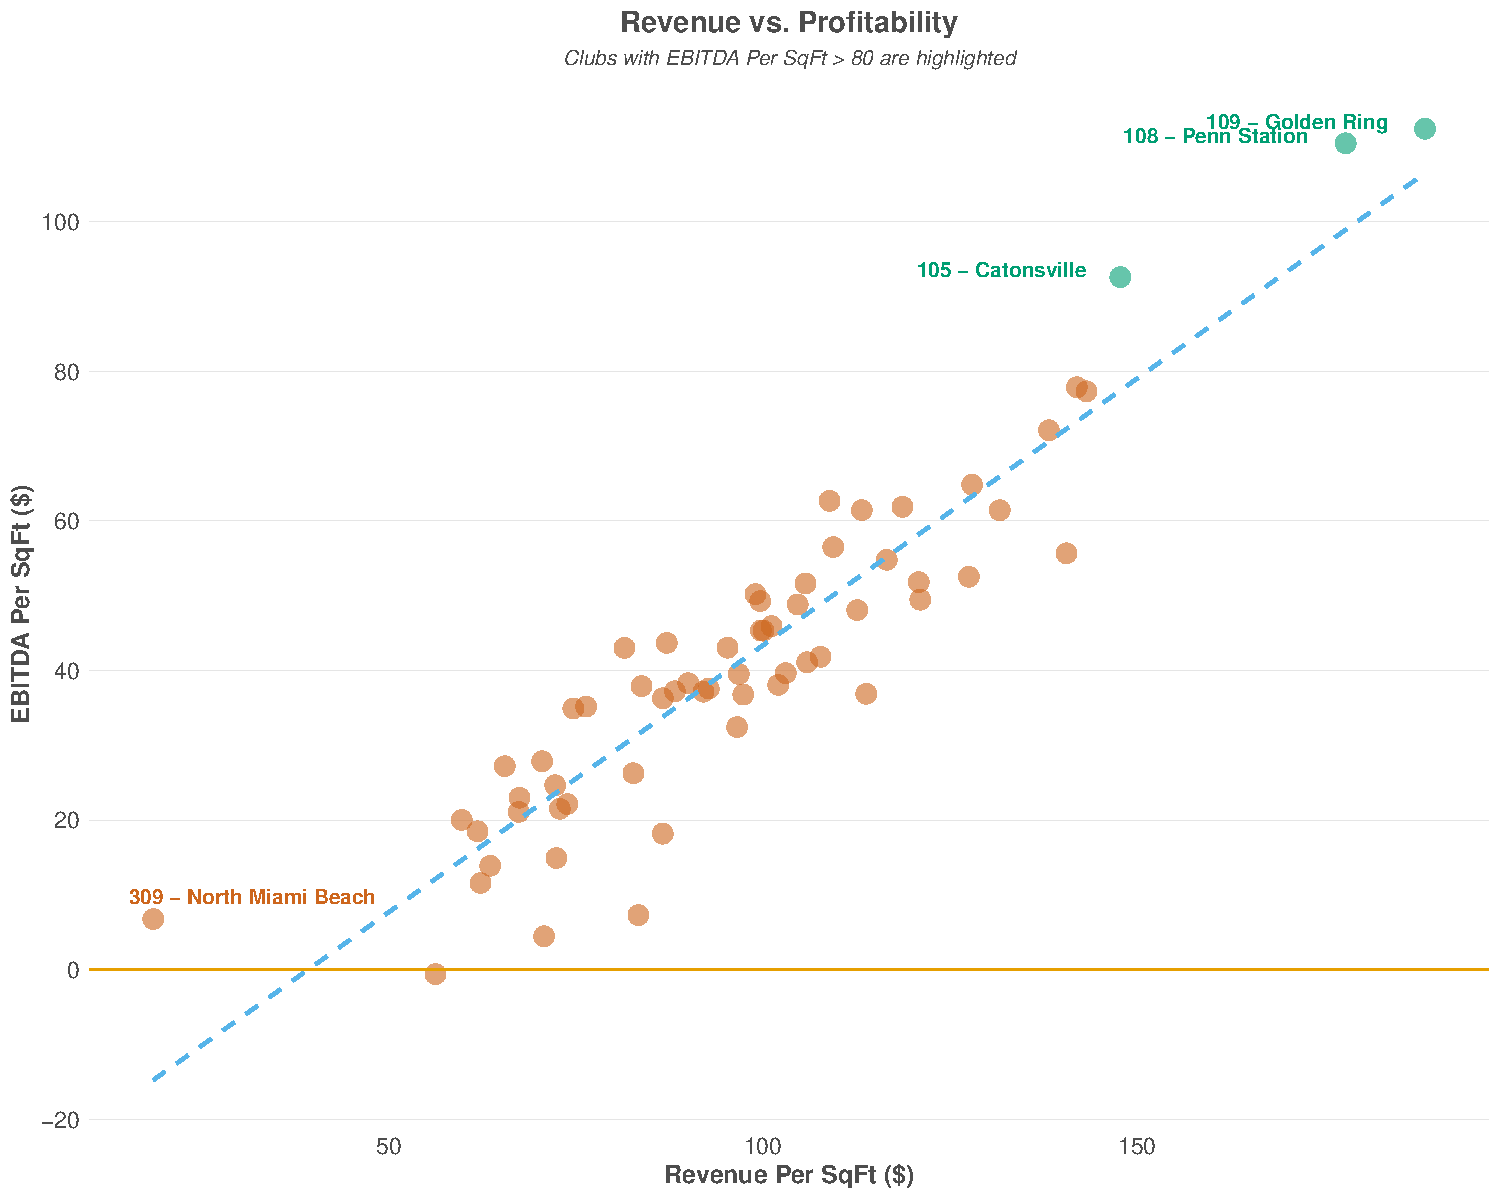
\includegraphics[keepaspectratio]{fit_report_profit_files/figure-pdf/scatter-revenue-eft-1.pdf}}

\subsection{Scatter Plot: Club Size vs Revenue Per
SqFt}\label{scatter-plot-club-size-vs-revenue-per-sqft}

\emph{Chart: Relationship between Club Size and Revenue (per sqft)}

\emph{Text: The most profitable clubs tend to be smaller in size.}

\begin{Shaded}
\begin{Highlighting}[]
\CommentTok{\# Scatterplot of RevenuePerSqFt vs. Size}
\FunctionTok{ggplot}\NormalTok{(}\FunctionTok{filter}\NormalTok{(club\_perf\_year4, RevenuePerSqFt }\SpecialCharTok{\textgreater{}} \DecValTok{40}\NormalTok{),}
       \FunctionTok{aes}\NormalTok{(}\AttributeTok{x =}\NormalTok{ Size, }\AttributeTok{y =}\NormalTok{ RevenuePerSqFt, }\AttributeTok{color =}\NormalTok{ EBITDAPerSqFtCat)) }\SpecialCharTok{+}
  \FunctionTok{geom\_point}\NormalTok{(}
    \AttributeTok{alpha =} \FloatTok{0.6}\NormalTok{,}
    \AttributeTok{size =} \DecValTok{4}
\NormalTok{  ) }\SpecialCharTok{+}
  \FunctionTok{scale\_color\_manual}\NormalTok{(}
    \AttributeTok{name =} \StringTok{"Profitability"}\NormalTok{,}
    \AttributeTok{values =} \FunctionTok{c}\NormalTok{(}\StringTok{"Low"} \OtherTok{=}\NormalTok{ custom\_palette[}\DecValTok{1}\NormalTok{], }\StringTok{"Medium"} \OtherTok{=}\NormalTok{ custom\_palette[}\DecValTok{2}\NormalTok{], }\StringTok{"High"} \OtherTok{=}\NormalTok{ custom\_palette[}\DecValTok{3}\NormalTok{])}
\NormalTok{  ) }\SpecialCharTok{+}
  \FunctionTok{geom\_hline}\NormalTok{(}
    \AttributeTok{yintercept =} \DecValTok{0}\NormalTok{,}
    \AttributeTok{color =}\NormalTok{ custom\_palette[}\DecValTok{2}\NormalTok{],}
    \AttributeTok{linetype =} \StringTok{"solid"}\NormalTok{,}
    \AttributeTok{linewidth =} \FloatTok{0.5}
\NormalTok{  ) }\SpecialCharTok{+}
  \FunctionTok{geom\_text}\NormalTok{(}
    \AttributeTok{data =}\NormalTok{ club\_perf\_year4 }\SpecialCharTok{\%\textgreater{}\%} \FunctionTok{filter}\NormalTok{(ClubNumber }\SpecialCharTok{\%in\%} \FunctionTok{c}\NormalTok{(}\DecValTok{105}\NormalTok{, }\DecValTok{108}\NormalTok{, }\DecValTok{109}\NormalTok{)),}
    \FunctionTok{aes}\NormalTok{(}\AttributeTok{x =}\NormalTok{ Size, }\AttributeTok{y =}\NormalTok{ RevenuePerSqFt, }\AttributeTok{label =} \FunctionTok{paste0}\NormalTok{(ClubName,}\StringTok{" {-} "}\NormalTok{, PopDensityType)),}
    \AttributeTok{hjust =} \FloatTok{0.1}\NormalTok{,}
    \AttributeTok{vjust =} \SpecialCharTok{{-}}\DecValTok{1}\NormalTok{,}
    \AttributeTok{color =}\NormalTok{ custom\_palette[}\DecValTok{3}\NormalTok{],}
    \AttributeTok{size =} \FloatTok{3.5}\NormalTok{,}
    \AttributeTok{fontface =} \StringTok{"bold"}
\NormalTok{  ) }\SpecialCharTok{+}
  \FunctionTok{geom\_smooth}\NormalTok{(}
    \AttributeTok{method =} \StringTok{"lm"}\NormalTok{,}
    \AttributeTok{se =} \ConstantTok{FALSE}\NormalTok{,}
    \AttributeTok{color =}\NormalTok{ custom\_palette[}\DecValTok{3}\NormalTok{],}
    \AttributeTok{linewidth =} \FloatTok{0.8}\NormalTok{,}
    \AttributeTok{linetype =} \StringTok{"dashed"}
\NormalTok{  ) }\SpecialCharTok{+}
  \FunctionTok{scale\_x\_continuous}\NormalTok{(}\AttributeTok{breaks =} \FunctionTok{seq}\NormalTok{(}\DecValTok{10000}\NormalTok{, }\DecValTok{34000}\NormalTok{, }\AttributeTok{by =} \DecValTok{2500}\NormalTok{)) }\SpecialCharTok{+}
  \FunctionTok{scale\_y\_continuous}\NormalTok{(}\AttributeTok{limits =} \FunctionTok{c}\NormalTok{(}\SpecialCharTok{{-}}\DecValTok{10}\NormalTok{, }\DecValTok{200}\NormalTok{)) }\SpecialCharTok{+}
  \FunctionTok{labs}\NormalTok{(}
    \AttributeTok{title =} \StringTok{"Are Bigger Clubs More Profitable?"}\NormalTok{,}
    \AttributeTok{subtitle =} \StringTok{"Excludes 309 {-} North Miami Beach"}\NormalTok{,}
    \AttributeTok{x =} \StringTok{"Club Size"}\NormalTok{,}
    \AttributeTok{y =} \StringTok{"Revenue Per SqFt ($)"}
\NormalTok{  ) }\SpecialCharTok{+}
  \FunctionTok{fit\_theme}\NormalTok{() }\SpecialCharTok{+}
  \FunctionTok{theme}\NormalTok{(}
    \AttributeTok{legend.position =} \StringTok{"right"}\NormalTok{,}
    \AttributeTok{panel.grid.major.x =} \FunctionTok{element\_line}\NormalTok{(}\AttributeTok{color =} \StringTok{"gray90"}\NormalTok{, }\AttributeTok{linewidth =} \FloatTok{0.2}\NormalTok{)}
\NormalTok{  )}
\end{Highlighting}
\end{Shaded}

\begin{verbatim}
`geom_smooth()` using formula = 'y ~ x'
\end{verbatim}

\pandocbounded{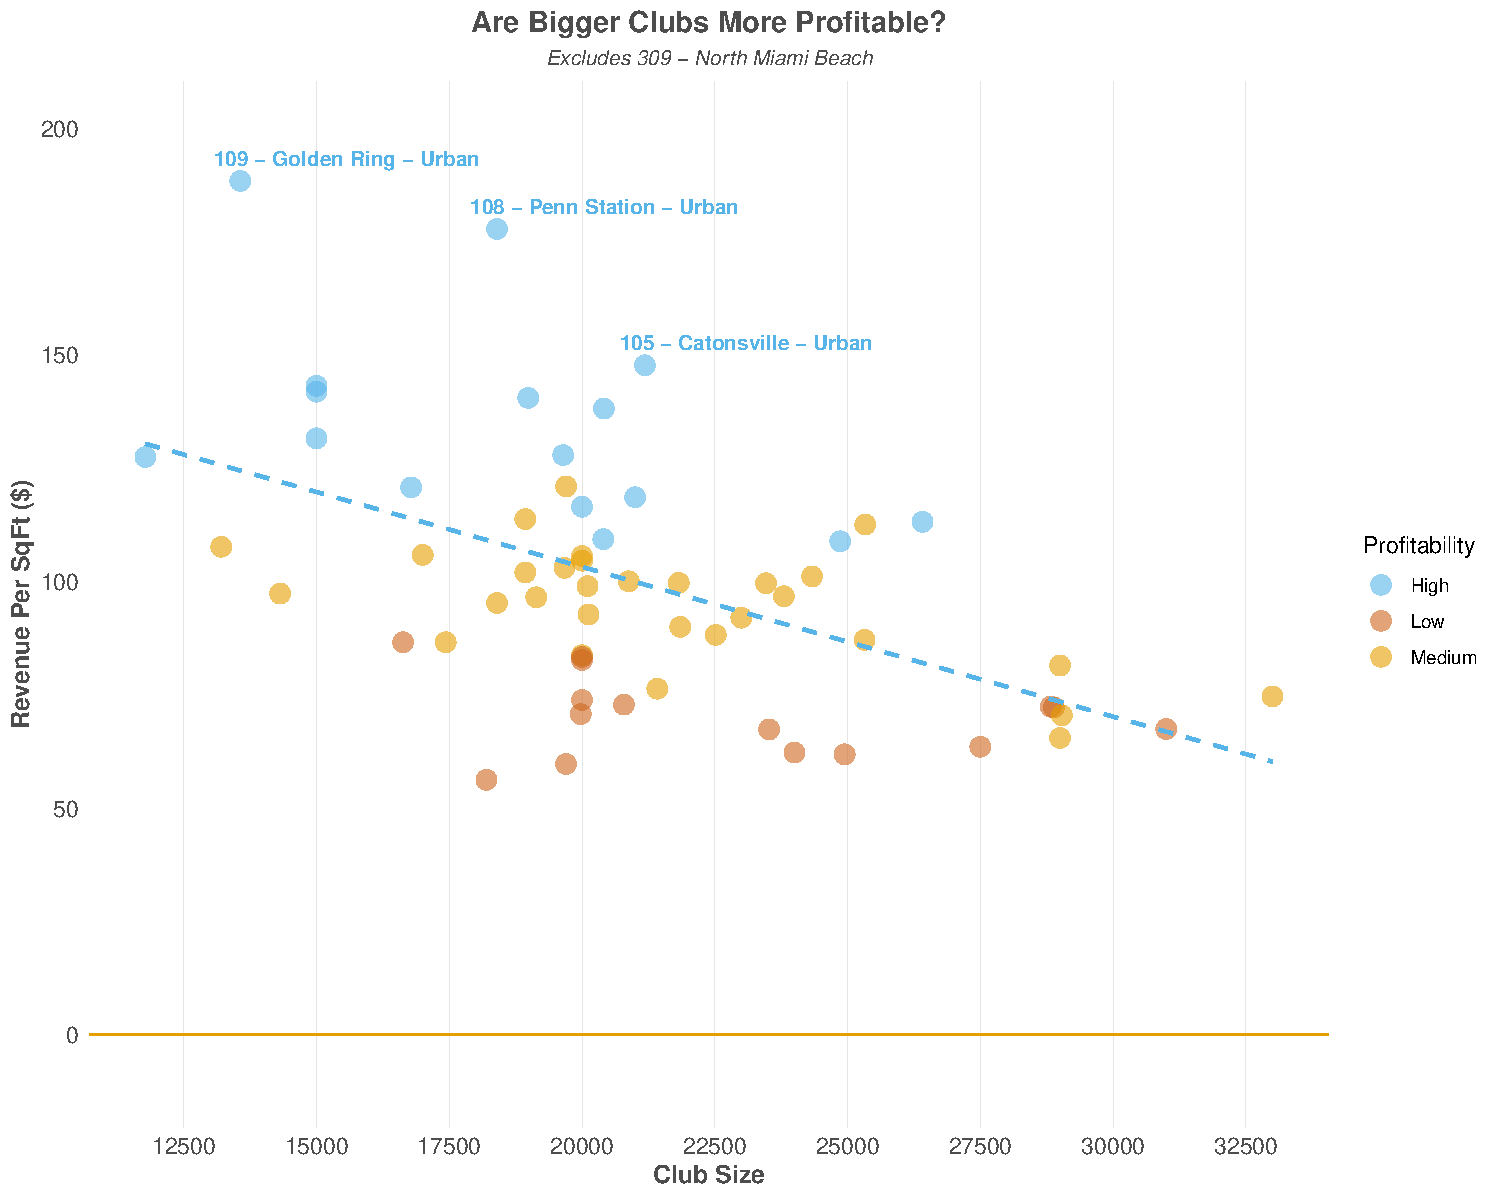
\includegraphics[keepaspectratio]{fit_report_profit_files/figure-pdf/scatter-size-revenue-1.pdf}}

\subsection{Boxplot: EBITDA PER SQFT, Mature Clubs (Year
4)}\label{boxplot-ebitda-per-sqft-mature-clubs-year-4}

\emph{Chart: Segmenting Mature Clubs by Profitability}

\emph{Text: We can group the clubs according to profitability using
percentiles: 25\% and 75\%. The three groups correspond to Low, Medium
and High profit clubs.}

\begin{Shaded}
\begin{Highlighting}[]
\CommentTok{\# Calculate median EBITDAPerSqFt for each category}
\NormalTok{median\_ebitda }\OtherTok{\textless{}{-}}\NormalTok{ club\_perf\_year4 }\SpecialCharTok{\%\textgreater{}\%}
  \FunctionTok{group\_by}\NormalTok{(EBITDAPerSqFtCat) }\SpecialCharTok{\%\textgreater{}\%}
  \FunctionTok{summarise}\NormalTok{(}\AttributeTok{MedianEBITDAPerSqFt =} \FunctionTok{median}\NormalTok{(EBITDAPerSqFt, }\AttributeTok{na.rm =} \ConstantTok{TRUE}\NormalTok{),}
            \AttributeTok{n =} \FunctionTok{n}\NormalTok{()}
\NormalTok{            ) }\SpecialCharTok{\%\textgreater{}\%}
  \FunctionTok{ungroup}\NormalTok{()}

\CommentTok{\# EBITDA Per SqFt}
\FunctionTok{ggplot}\NormalTok{(club\_perf\_year4, }\FunctionTok{aes}\NormalTok{(}\AttributeTok{x =}\NormalTok{ EBITDAPerSqFt, }\AttributeTok{y =}\NormalTok{ EBITDAPerSqFtCat, }\AttributeTok{fill =}\NormalTok{ EBITDAPerSqFtCat)) }\SpecialCharTok{+}
  \FunctionTok{geom\_boxplot}\NormalTok{() }\SpecialCharTok{+}
  \FunctionTok{geom\_point}\NormalTok{(}\AttributeTok{position =} \FunctionTok{position\_jitter}\NormalTok{(}\AttributeTok{height =} \FloatTok{0.1}\NormalTok{), }\AttributeTok{alpha =} \FloatTok{0.5}\NormalTok{, }\AttributeTok{color =} \StringTok{"gray52"}\NormalTok{) }\SpecialCharTok{+}
  \CommentTok{\# Annotate median values below the boxplots}
  \FunctionTok{geom\_text}\NormalTok{(}
    \AttributeTok{data =}\NormalTok{ median\_ebitda,}
    \FunctionTok{aes}\NormalTok{(}
      \AttributeTok{x =}\NormalTok{ MedianEBITDAPerSqFt,}
      \AttributeTok{y =}\NormalTok{ EBITDAPerSqFtCat,}
      \AttributeTok{label =} \FunctionTok{paste0}\NormalTok{(}\StringTok{"$"}\NormalTok{, }\FunctionTok{round}\NormalTok{(MedianEBITDAPerSqFt, }\DecValTok{0}\NormalTok{))}
\NormalTok{    ),}
    \AttributeTok{vjust =} \SpecialCharTok{{-}}\FloatTok{5.4}\NormalTok{,}
    \AttributeTok{hjust =} \FloatTok{0.5}\NormalTok{,}
    \AttributeTok{color =} \StringTok{"gray30"}\NormalTok{,}
    \AttributeTok{size =} \FloatTok{3.5}\NormalTok{,}
    \AttributeTok{fontface =} \StringTok{"bold"}
\NormalTok{  ) }\SpecialCharTok{+}
  \FunctionTok{geom\_text}\NormalTok{(}
    \AttributeTok{data =}\NormalTok{ median\_ebitda,}
    \FunctionTok{aes}\NormalTok{(}
      \AttributeTok{x =} \DecValTok{120}\NormalTok{,}
      \AttributeTok{y =}\NormalTok{ EBITDAPerSqFtCat,}
      \AttributeTok{label =} \FunctionTok{paste0}\NormalTok{(}\StringTok{"n = "}\NormalTok{, n)}
\NormalTok{    ),}
    \AttributeTok{color =} \StringTok{"grey60"}\NormalTok{,}
    \AttributeTok{size =} \FloatTok{4.5}\NormalTok{,}
    \AttributeTok{fontface =} \StringTok{"bold"}
\NormalTok{  ) }\SpecialCharTok{+}
  \FunctionTok{labs}\NormalTok{(}
    \AttributeTok{title =} \StringTok{"Segmentation by Profitability {-} Mature Clubs"}\NormalTok{,}
    \AttributeTok{subtitle =} \StringTok{"Values shown for the Average Club"}\NormalTok{,}
    \AttributeTok{x =} \StringTok{"EBITDA Per SqFt"}\NormalTok{,}
    \AttributeTok{y =} \StringTok{"Category"}
\NormalTok{  ) }\SpecialCharTok{+}
  \FunctionTok{scale\_y\_discrete}\NormalTok{(}\AttributeTok{limits =} \FunctionTok{c}\NormalTok{(}\StringTok{"Low"}\NormalTok{, }\StringTok{"Medium"}\NormalTok{, }\StringTok{"High"}\NormalTok{)) }\SpecialCharTok{+}
  \FunctionTok{scale\_fill\_manual}\NormalTok{(}\AttributeTok{values =}\NormalTok{ custom\_palette) }\SpecialCharTok{+}
  \FunctionTok{scale\_x\_continuous}\NormalTok{(}\AttributeTok{labels =} \ControlFlowTok{function}\NormalTok{(x) }\FunctionTok{paste0}\NormalTok{(}\StringTok{"$"}\NormalTok{, }\FunctionTok{round}\NormalTok{(x, }\DecValTok{1}\NormalTok{))) }\SpecialCharTok{+}
  \FunctionTok{fit\_theme}\NormalTok{()}
\end{Highlighting}
\end{Shaded}

\pandocbounded{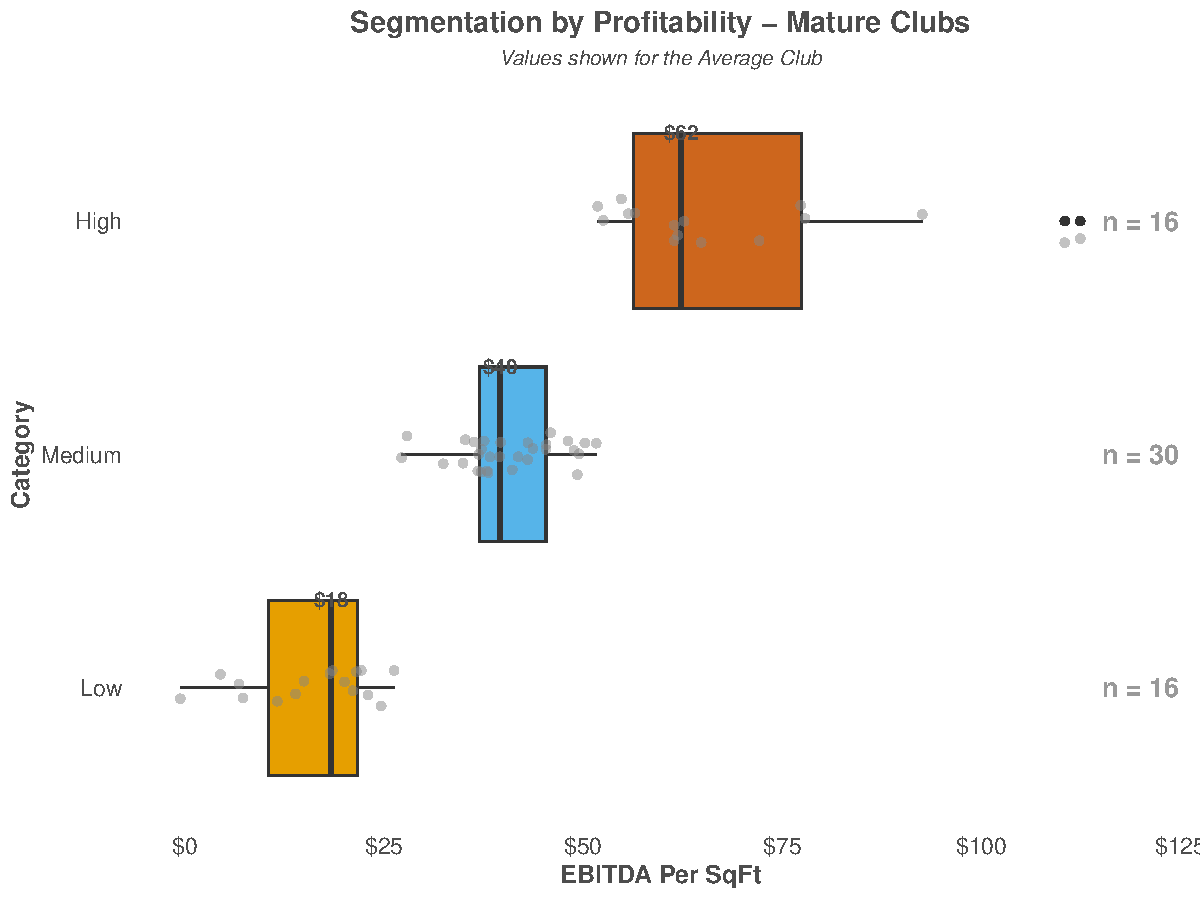
\includegraphics[keepaspectratio]{fit_report_profit_files/figure-pdf/boxplot-ebitda-1.pdf}}

\emph{Clubs with EBITDA close to zero} * 301 - Coconut Creek, FL\emph{ }
303 - Pompano, FL\emph{ } 309 - North Miami Beach, FL\emph{ } 128 - Penn
Branch, DC*

\subsection{Performance Metrics: Growth \% Years 0-4, Mature Clubs (Year
4)}\label{performance-metrics-growth-years-0-4-mature-clubs-year-4}

\emph{Chart: Segmenting Mature Clubs by Growth \%}

\emph{Text: Clubs are also grouped by Growth \% using the same
percentiles: 25\% and 75\%.}

\begin{Shaded}
\begin{Highlighting}[]
\CommentTok{\# Calculate median Growth \% 04 for each category}
\NormalTok{median\_cagryears04 }\OtherTok{\textless{}{-}}\NormalTok{ club\_perf\_year4 }\SpecialCharTok{\%\textgreater{}\%}
  \FunctionTok{filter}\NormalTok{(}\SpecialCharTok{!}\FunctionTok{is.na}\NormalTok{(CAGRYears04)) }\SpecialCharTok{\%\textgreater{}\%}
  \FunctionTok{group\_by}\NormalTok{(CAGRYears04Cat) }\SpecialCharTok{\%\textgreater{}\%}
  \FunctionTok{summarise}\NormalTok{(}\AttributeTok{MedianCAGRYears04 =} \FunctionTok{median}\NormalTok{(CAGRYears04, }\AttributeTok{na.rm =} \ConstantTok{TRUE}\NormalTok{),}
            \AttributeTok{n =} \FunctionTok{n}\NormalTok{()}
\NormalTok{            ) }\SpecialCharTok{\%\textgreater{}\%}
  \FunctionTok{ungroup}\NormalTok{()}

\CommentTok{\# Subset to records where CAGRYears47 is not NULL and exclude 309 {-} Miami Beach (low revenue)}
\NormalTok{plot\_data }\OtherTok{\textless{}{-}}\NormalTok{ club\_perf\_year4 }\SpecialCharTok{\%\textgreater{}\%}
  \FunctionTok{filter}\NormalTok{(}\SpecialCharTok{!}\FunctionTok{is.na}\NormalTok{(CAGRYears04))}

\CommentTok{\# Growth \% (Years 0{-}4)}
\FunctionTok{ggplot}\NormalTok{(plot\_data, }\FunctionTok{aes}\NormalTok{(}\AttributeTok{x =}\NormalTok{ CAGRYears04, }\AttributeTok{y =}\NormalTok{ CAGRYears04Cat, }\AttributeTok{fill =}\NormalTok{ CAGRYears04Cat)) }\SpecialCharTok{+}
  \FunctionTok{geom\_boxplot}\NormalTok{() }\SpecialCharTok{+}
  \FunctionTok{geom\_point}\NormalTok{(}\AttributeTok{position =} \FunctionTok{position\_jitter}\NormalTok{(}\AttributeTok{height =} \FloatTok{0.1}\NormalTok{), }
             \AttributeTok{alpha =} \FloatTok{0.5}\NormalTok{, }
             \AttributeTok{color =} \StringTok{"gray52"}\NormalTok{) }\SpecialCharTok{+}
  \CommentTok{\# Annotate median values below the boxplots}
  \FunctionTok{geom\_text}\NormalTok{(}
    \AttributeTok{data =}\NormalTok{ median\_cagryears04,}
    \FunctionTok{aes}\NormalTok{(}
      \AttributeTok{x =}\NormalTok{ MedianCAGRYears04,}
      \AttributeTok{y =}\NormalTok{ CAGRYears04Cat,}
      \AttributeTok{label =} \FunctionTok{paste0}\NormalTok{(}\FunctionTok{round}\NormalTok{(MedianCAGRYears04}\SpecialCharTok{*}\DecValTok{100}\NormalTok{, }\DecValTok{0}\NormalTok{), }\StringTok{"\%"}\NormalTok{)}
\NormalTok{    ),}
    \AttributeTok{vjust =} \SpecialCharTok{{-}}\FloatTok{5.4}\NormalTok{,}
    \AttributeTok{hjust =} \FloatTok{0.5}\NormalTok{,}
    \AttributeTok{color =} \StringTok{"gray30"}\NormalTok{,}
    \AttributeTok{size =} \FloatTok{3.5}\NormalTok{,}
    \AttributeTok{fontface =} \StringTok{"bold"}
\NormalTok{  ) }\SpecialCharTok{+}
  \FunctionTok{geom\_text}\NormalTok{(}
    \AttributeTok{data =}\NormalTok{ median\_cagryears04,}
    \FunctionTok{aes}\NormalTok{(}
      \AttributeTok{x =}\NormalTok{ .}\DecValTok{22}\NormalTok{,}
      \AttributeTok{y =}\NormalTok{ CAGRYears04Cat,}
      \AttributeTok{label =} \FunctionTok{paste0}\NormalTok{(}\StringTok{"n = "}\NormalTok{, n)}
\NormalTok{    ),}
    \AttributeTok{color =} \StringTok{"grey60"}\NormalTok{,}
    \AttributeTok{size =} \FloatTok{4.5}\NormalTok{,}
    \AttributeTok{fontface =} \StringTok{"bold"}
\NormalTok{  ) }\SpecialCharTok{+}
  \FunctionTok{labs}\NormalTok{(}
    \AttributeTok{title =} \StringTok{"Segmentation by Growth \% {-} Mature Clubs"}\NormalTok{,}
    \AttributeTok{subtitle =}\NormalTok{ (}\StringTok{"Growth \% shown for the Average Club in each Category"}\NormalTok{),}
    \AttributeTok{x =} \StringTok{"Growth \% (Years 0{-}4)"}\NormalTok{,}
    \AttributeTok{y =} \StringTok{"Category"}
\NormalTok{  ) }\SpecialCharTok{+}
  \FunctionTok{scale\_y\_discrete}\NormalTok{(}\AttributeTok{limits =} \FunctionTok{c}\NormalTok{(}\StringTok{"Low"}\NormalTok{, }\StringTok{"Medium"}\NormalTok{, }\StringTok{"High"}\NormalTok{)) }\SpecialCharTok{+}
  \FunctionTok{scale\_fill\_manual}\NormalTok{(}\AttributeTok{values =}\NormalTok{ custom\_palette) }\SpecialCharTok{+}
  \FunctionTok{scale\_x\_continuous}\NormalTok{(}\AttributeTok{labels =} \ControlFlowTok{function}\NormalTok{(x) }\FunctionTok{paste0}\NormalTok{(}\FunctionTok{round}\NormalTok{(x}\SpecialCharTok{*}\DecValTok{100}\NormalTok{, }\DecValTok{0}\NormalTok{), }\StringTok{"\%"}\NormalTok{)) }\SpecialCharTok{+}
  \FunctionTok{fit\_theme}\NormalTok{()}
\end{Highlighting}
\end{Shaded}

\pandocbounded{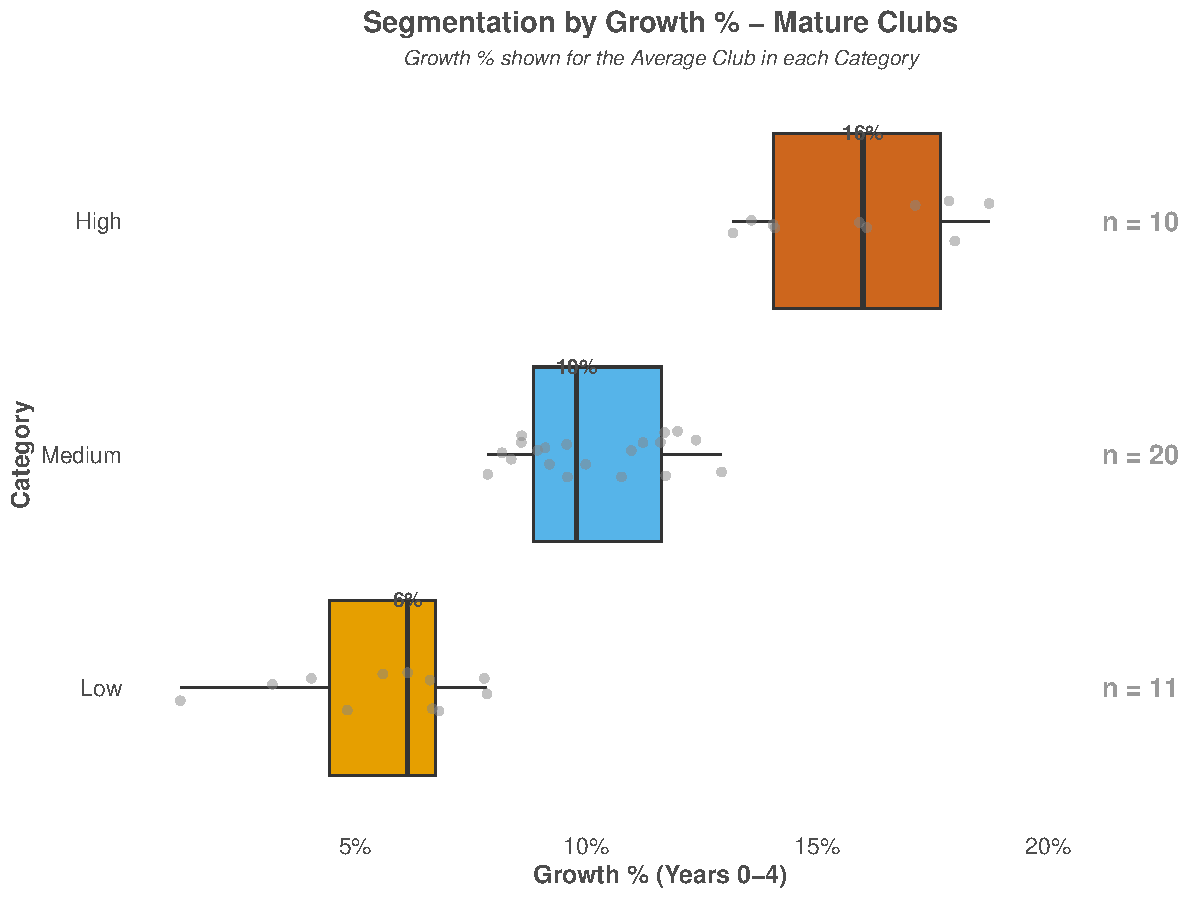
\includegraphics[keepaspectratio]{fit_report_profit_files/figure-pdf/boxplot-growth-1.pdf}}

\subsection{Matrix: Growth \% (Years 0-4) vs EBITDA PER
SQFT}\label{matrix-growth-years-0-4-vs-ebitda-per-sqft}

\emph{Chart: Matrix of clubs along Profitability and Growth \%}

\emph{Text: Only two clubs hit the sweet spot of high growth and high
profitability}

\begin{Shaded}
\begin{Highlighting}[]
\CommentTok{\# Subset to records where CAGRYears47 is not NULL and exclude 309 {-} Miami Beach (low revenue)}
\NormalTok{plot\_data }\OtherTok{\textless{}{-}}\NormalTok{ club\_perf\_year4 }\SpecialCharTok{\%\textgreater{}\%}
  \FunctionTok{filter}\NormalTok{(}\SpecialCharTok{!}\FunctionTok{is.na}\NormalTok{(CAGRYears04) }\SpecialCharTok{\&}\NormalTok{ RevenuePerSqFt }\SpecialCharTok{\textgreater{}} \DecValTok{40}\NormalTok{)}

\CommentTok{\# Calculate 75 percentiles}
\NormalTok{perc75\_cagr }\OtherTok{\textless{}{-}}\NormalTok{ plot\_data }\SpecialCharTok{\%\textgreater{}\%}
  \FunctionTok{filter}\NormalTok{(CAGRYears04Cat }\SpecialCharTok{==} \StringTok{"High"}\NormalTok{) }\SpecialCharTok{\%\textgreater{}\%}
  \FunctionTok{summarise}\NormalTok{(}
    \AttributeTok{min\_cagr =} \FunctionTok{min}\NormalTok{(CAGRYears04, }\AttributeTok{na.rm =} \ConstantTok{TRUE}\NormalTok{)}
\NormalTok{  ) }\SpecialCharTok{\%\textgreater{}\%}
  \FunctionTok{pull}\NormalTok{(min\_cagr)}

\NormalTok{perc75\_ebitda }\OtherTok{\textless{}{-}}\NormalTok{ plot\_data }\SpecialCharTok{\%\textgreater{}\%}
  \FunctionTok{filter}\NormalTok{(EBITDAPerSqFtCat }\SpecialCharTok{==} \StringTok{"High"}\NormalTok{) }\SpecialCharTok{\%\textgreater{}\%}
  \FunctionTok{summarise}\NormalTok{(}
    \AttributeTok{min\_ebitda =} \FunctionTok{min}\NormalTok{(EBITDAPerSqFt, }\AttributeTok{na.rm =} \ConstantTok{TRUE}\NormalTok{)}
\NormalTok{  ) }\SpecialCharTok{\%\textgreater{}\%}
  \FunctionTok{pull}\NormalTok{(min\_ebitda)}

\CommentTok{\# Create Plot}
\FunctionTok{ggplot}\NormalTok{(plot\_data }\SpecialCharTok{\%\textgreater{}\%} \FunctionTok{filter}\NormalTok{(EBITDAPerSqFt }\SpecialCharTok{\textless{}}\NormalTok{ perc75\_ebitda }\SpecialCharTok{|}\NormalTok{ CAGRYears04 }\SpecialCharTok{\textless{}}\NormalTok{ perc75\_cagr),}
       \FunctionTok{aes}\NormalTok{(}\AttributeTok{x =}\NormalTok{ CAGRYears04, }\AttributeTok{y =}\NormalTok{ EBITDAPerSqFt, }\AttributeTok{label =}\NormalTok{ ClubNumber)) }\SpecialCharTok{+}
  \FunctionTok{geom\_point}\NormalTok{(}\AttributeTok{color =}\NormalTok{ custom\_palette[}\DecValTok{1}\NormalTok{], }
             \AttributeTok{alpha =} \FloatTok{0.7}\NormalTok{, }
             \AttributeTok{size =} \DecValTok{4}\NormalTok{) }\SpecialCharTok{+}
  \FunctionTok{geom\_text}\NormalTok{(}\AttributeTok{vjust =} \SpecialCharTok{{-}}\FloatTok{0.8}\NormalTok{, }
            \AttributeTok{size =} \DecValTok{4}\NormalTok{, }
            \AttributeTok{color =}\NormalTok{ custom\_palette[}\DecValTok{2}\NormalTok{]}
\NormalTok{            ) }\SpecialCharTok{+}
  \FunctionTok{geom\_hline}\NormalTok{(}\AttributeTok{yintercept =}\NormalTok{ perc75\_ebitda, }
             \AttributeTok{linetype =} \StringTok{"dashed"}\NormalTok{, }
             \AttributeTok{color =}\NormalTok{ custom\_palette[}\DecValTok{3}\NormalTok{]}
\NormalTok{             ) }\SpecialCharTok{+}
  \FunctionTok{geom\_vline}\NormalTok{(}\AttributeTok{xintercept =}\NormalTok{ perc75\_cagr, }
             \AttributeTok{linetype =} \StringTok{"dashed"}\NormalTok{, }
             \AttributeTok{color =}\NormalTok{ custom\_palette[}\DecValTok{3}\NormalTok{]}
\NormalTok{             ) }\SpecialCharTok{+}
  \FunctionTok{annotate}\NormalTok{(}\StringTok{"text"}\NormalTok{, }\AttributeTok{x =}\NormalTok{ perc75\_cagr, }\AttributeTok{y =} \DecValTok{100}\NormalTok{,}
           \AttributeTok{label =} \StringTok{"{-}\textgreater{} High Growth"}\NormalTok{,}
           \AttributeTok{hjust =} \SpecialCharTok{{-}}\FloatTok{0.2}\NormalTok{,}
           \AttributeTok{vjust =} \DecValTok{0}\NormalTok{,}
           \AttributeTok{color =}\NormalTok{ custom\_palette[}\DecValTok{3}\NormalTok{],}
           \AttributeTok{size =} \FloatTok{3.5}\NormalTok{,}
           \AttributeTok{fontface =} \StringTok{"bold"}
\NormalTok{           ) }\SpecialCharTok{+}
  \FunctionTok{annotate}\NormalTok{(}\StringTok{"text"}\NormalTok{, }\AttributeTok{x =} \SpecialCharTok{{-}}\FloatTok{0.05}\NormalTok{, }\AttributeTok{y =}\NormalTok{ perc75\_ebitda, }\AttributeTok{na.rm =} \ConstantTok{TRUE}\NormalTok{,}
           \AttributeTok{label =} \StringTok{"\^{} High Profitability"}\NormalTok{,}
           \AttributeTok{hjust =} \FloatTok{0.2}\NormalTok{,}
           \AttributeTok{vjust =} \SpecialCharTok{{-}}\FloatTok{1.2}\NormalTok{,}
           \AttributeTok{color =}\NormalTok{ custom\_palette[}\DecValTok{3}\NormalTok{],}
           \AttributeTok{size =} \FloatTok{3.5}\NormalTok{,}
           \AttributeTok{fontface =} \StringTok{"bold"}\NormalTok{) }\SpecialCharTok{+}
  \FunctionTok{geom\_point}\NormalTok{(}\AttributeTok{data =}\NormalTok{ plot\_data }\SpecialCharTok{\%\textgreater{}\%} \FunctionTok{filter}\NormalTok{(EBITDAPerSqFt }\SpecialCharTok{\textgreater{}=}\NormalTok{ perc75\_ebitda }\SpecialCharTok{\&}\NormalTok{ CAGRYears04 }\SpecialCharTok{\textgreater{}=}\NormalTok{ perc75\_cagr),}
             \FunctionTok{aes}\NormalTok{(}\AttributeTok{x =}\NormalTok{ CAGRYears04, }\AttributeTok{y =}\NormalTok{ EBITDAPerSqFt),}
             \AttributeTok{color =}\NormalTok{ custom\_palette[}\DecValTok{1}\NormalTok{], }
             \AttributeTok{alpha =} \FloatTok{0.7}\NormalTok{, }
             \AttributeTok{size =} \DecValTok{4}\NormalTok{) }\SpecialCharTok{+}
  \FunctionTok{geom\_text}\NormalTok{(}
          \AttributeTok{data =}\NormalTok{ plot\_data }\SpecialCharTok{\%\textgreater{}\%} \FunctionTok{filter}\NormalTok{(EBITDAPerSqFt }\SpecialCharTok{\textgreater{}=}\NormalTok{ perc75\_ebitda }\SpecialCharTok{\&}\NormalTok{ CAGRYears04 }\SpecialCharTok{\textgreater{}=}\NormalTok{ perc75\_cagr),}
          \FunctionTok{aes}\NormalTok{(}\AttributeTok{x =}\NormalTok{ CAGRYears04, }\AttributeTok{y =}\NormalTok{ EBITDAPerSqFt, }\AttributeTok{label =}\NormalTok{ ClubName),}
          \AttributeTok{vjust =} \SpecialCharTok{{-}}\FloatTok{0.8}\NormalTok{,}
          \AttributeTok{size =} \DecValTok{4}\NormalTok{,}
          \AttributeTok{color =}\NormalTok{ custom\_palette[}\DecValTok{2}\NormalTok{]}
\NormalTok{  ) }\SpecialCharTok{+}
  \FunctionTok{scale\_x\_continuous}\NormalTok{(}\AttributeTok{labels =}\NormalTok{ percent, }\AttributeTok{limits =} \FunctionTok{c}\NormalTok{(}\SpecialCharTok{{-}}\FloatTok{0.07}\NormalTok{, }\FloatTok{0.26}\NormalTok{)) }\SpecialCharTok{+}
  \FunctionTok{scale\_y\_continuous}\NormalTok{(}\AttributeTok{limits =} \FunctionTok{c}\NormalTok{(}\SpecialCharTok{{-}}\DecValTok{10}\NormalTok{, }\DecValTok{100}\NormalTok{)) }\SpecialCharTok{+}
  \FunctionTok{labs}\NormalTok{(}
    \AttributeTok{title =} \StringTok{"Growth \% vs Profitabilty Matrix"}\NormalTok{,}
    \AttributeTok{subtitle =} \StringTok{"Mature Clubs"}\NormalTok{,}
    \AttributeTok{x =} \StringTok{"Growth \% (Years 0{-}4)"}\NormalTok{,}
    \AttributeTok{y =} \StringTok{"EBITDA Per SqFt ($)"}
\NormalTok{  ) }\SpecialCharTok{+}
  \FunctionTok{fit\_theme}\NormalTok{()}
\end{Highlighting}
\end{Shaded}

\pandocbounded{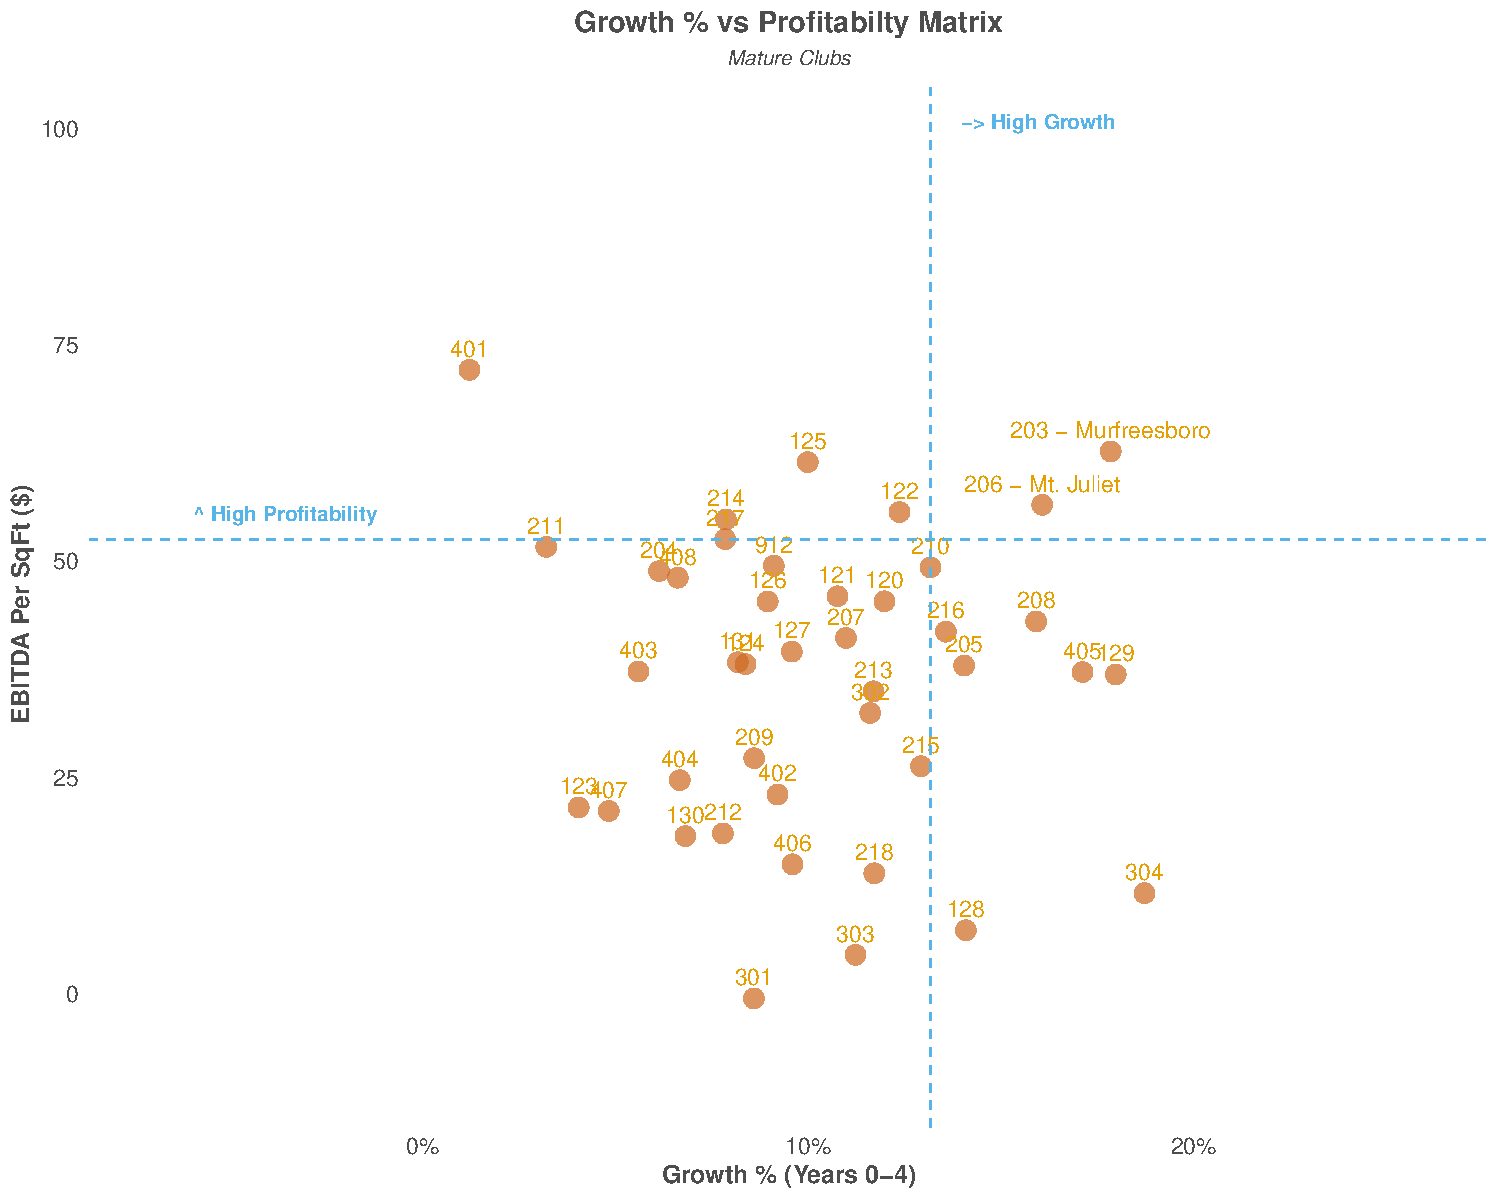
\includegraphics[keepaspectratio]{fit_report_profit_files/figure-pdf/matrix-growth-profit-1.pdf}}

\subsection{EBITDA PER SQFT and Growth \%: Top
Clubs}\label{ebitda-per-sqft-and-growth-top-clubs}

\emph{Chart: List of Top Clubs according to Profitability and Growth \%}

\emph{Text: High-profit clubs have EBITDA (per sqft) above \$50. In the
case of Growth \%, top clubs have double-digit growth rates (Years 0-4)
of active members.}

\begin{Shaded}
\begin{Highlighting}[]
\NormalTok{med\_cagr }\OtherTok{\textless{}{-}}\NormalTok{ plot\_data }\SpecialCharTok{\%\textgreater{}\%}
  \FunctionTok{summarise}\NormalTok{(}
    \AttributeTok{med\_cagr =} \FunctionTok{mean}\NormalTok{(CAGRYears04, }\AttributeTok{na.rm =} \ConstantTok{TRUE}\NormalTok{)}
\NormalTok{  ) }\SpecialCharTok{\%\textgreater{}\%}
  \FunctionTok{pull}\NormalTok{(med\_cagr)}

\NormalTok{med\_ebitda }\OtherTok{\textless{}{-}}\NormalTok{ plot\_data }\SpecialCharTok{\%\textgreater{}\%}
  \FunctionTok{summarise}\NormalTok{(}
    \AttributeTok{med\_ebitda =} \FunctionTok{median}\NormalTok{(EBITDAPerSqFt, }\AttributeTok{na.rm =} \ConstantTok{TRUE}\NormalTok{)}
\NormalTok{  ) }\SpecialCharTok{\%\textgreater{}\%}
  \FunctionTok{pull}\NormalTok{(med\_ebitda)}

\CommentTok{\# {-}{-}{-} Chart 1: EBITDA per SqFt {-}{-}{-}}
\NormalTok{ebitda\_persqt\_sorted }\OtherTok{\textless{}{-}}\NormalTok{ club\_perf\_year4 }\SpecialCharTok{\%\textgreater{}\%}
  \FunctionTok{filter}\NormalTok{(}\SpecialCharTok{!}\FunctionTok{is.na}\NormalTok{(CAGRYears04) }\SpecialCharTok{\&}\NormalTok{ RevenuePerSqFt }\SpecialCharTok{\textgreater{}} \DecValTok{40}\NormalTok{) }\SpecialCharTok{\%\textgreater{}\%}
  \FunctionTok{filter}\NormalTok{(EBITDAPerSqFtCat }\SpecialCharTok{==} \StringTok{"High"}\NormalTok{) }\SpecialCharTok{\%\textgreater{}\%}
  \FunctionTok{arrange}\NormalTok{(EBITDAPerSqFt)}

\NormalTok{p1 }\OtherTok{\textless{}{-}} \FunctionTok{ggplot}\NormalTok{(ebitda\_persqt\_sorted, }\FunctionTok{aes}\NormalTok{(}\AttributeTok{x =}\NormalTok{ EBITDAPerSqFt, }
                                       \AttributeTok{y =} \FunctionTok{reorder}\NormalTok{(ClubName, EBITDAPerSqFt))}
\NormalTok{             ) }\SpecialCharTok{+}
  \FunctionTok{geom\_point}\NormalTok{(}\AttributeTok{size =} \DecValTok{4}\NormalTok{, }
             \AttributeTok{alpha =} \FloatTok{0.8}\NormalTok{, }
             \AttributeTok{color =}\NormalTok{ custom\_palette[}\DecValTok{1}\NormalTok{]) }\SpecialCharTok{+}
  \FunctionTok{geom\_segment}\NormalTok{(}\FunctionTok{aes}\NormalTok{(}\AttributeTok{x =} \DecValTok{0}\NormalTok{, }
                   \AttributeTok{xend =}\NormalTok{ EBITDAPerSqFt, }
                   \AttributeTok{yend =} \FunctionTok{reorder}\NormalTok{(ClubName, EBITDAPerSqFt)}
\NormalTok{                   ),}
               \AttributeTok{color =}\NormalTok{ custom\_palette[}\DecValTok{1}\NormalTok{], }
               \AttributeTok{alpha =} \FloatTok{0.4}\NormalTok{) }\SpecialCharTok{+}
  \FunctionTok{scale\_x\_continuous}\NormalTok{(}\AttributeTok{labels =} \ControlFlowTok{function}\NormalTok{(x) }\FunctionTok{paste0}\NormalTok{(}\StringTok{"$"}\NormalTok{, }\FunctionTok{round}\NormalTok{(x, }\DecValTok{1}\NormalTok{)), }
                     \AttributeTok{limits =} \FunctionTok{c}\NormalTok{(}\DecValTok{0}\NormalTok{, }\DecValTok{100}\NormalTok{)}
\NormalTok{  ) }\SpecialCharTok{+}
  \FunctionTok{geom\_vline}\NormalTok{(}\AttributeTok{xintercept =}\NormalTok{ med\_ebitda, }
             \AttributeTok{linetype =} \StringTok{"dashed"}\NormalTok{, }
             \AttributeTok{color =}\NormalTok{ custom\_palette[}\DecValTok{3}\NormalTok{], }
             \AttributeTok{linewidth =} \FloatTok{0.8}
\NormalTok{             ) }\SpecialCharTok{+}
  \FunctionTok{annotate}\NormalTok{(}\StringTok{"text"}\NormalTok{, }
           \AttributeTok{x =}\NormalTok{ med\_ebitda, }
           \AttributeTok{y =} \ConstantTok{Inf}\NormalTok{, }
           \AttributeTok{na.rm =} \ConstantTok{TRUE}\NormalTok{,}
           \AttributeTok{label =} \FunctionTok{paste0}\NormalTok{(}\StringTok{"Avg Club: $"}\NormalTok{, med\_ebitda),}
           \AttributeTok{hjust =} \SpecialCharTok{{-}}\FloatTok{0.06}\NormalTok{, }
           \AttributeTok{vjust =} \FloatTok{1.2}\NormalTok{, }
           \AttributeTok{color =}\NormalTok{ custom\_palette[}\DecValTok{3}\NormalTok{], }
           \AttributeTok{size =} \FloatTok{3.5}\NormalTok{, }
           \AttributeTok{fontface =} \StringTok{"bold"}\NormalTok{) }\SpecialCharTok{+}
  \FunctionTok{labs}\NormalTok{(}
    \AttributeTok{title =} \StringTok{"High Profitability Clubs"}\NormalTok{,}
    \AttributeTok{subtitle =} \StringTok{"Mature Clubs {-} Y4"}\NormalTok{,}
    \AttributeTok{x =} \StringTok{""}\NormalTok{,}
    \AttributeTok{y =} \StringTok{""}
\NormalTok{  ) }\SpecialCharTok{+}
  \FunctionTok{fit\_theme}\NormalTok{() }\SpecialCharTok{+}
  \FunctionTok{theme}\NormalTok{(}
    \AttributeTok{panel.grid.major.x =} \FunctionTok{element\_line}\NormalTok{(}\AttributeTok{color =} \StringTok{"gray90"}\NormalTok{, }\AttributeTok{linewidth =} \FloatTok{0.2}\NormalTok{)}
\NormalTok{  )}

\CommentTok{\# {-}{-}{-} Chart 2: CAGR Years 4{-}7 {-}{-}{-}}
\NormalTok{cagr\_year4\_sorted }\OtherTok{\textless{}{-}}\NormalTok{ club\_perf\_year4 }\SpecialCharTok{\%\textgreater{}\%}
  \FunctionTok{filter}\NormalTok{(}\SpecialCharTok{!}\FunctionTok{is.na}\NormalTok{(CAGRYears04) }\SpecialCharTok{\&}\NormalTok{ RevenuePerSqFt }\SpecialCharTok{\textgreater{}} \DecValTok{40}\NormalTok{) }\SpecialCharTok{\%\textgreater{}\%}
  \FunctionTok{filter}\NormalTok{(CAGRYears04Cat }\SpecialCharTok{==} \StringTok{"High"}\NormalTok{) }\SpecialCharTok{\%\textgreater{}\%}
  \FunctionTok{arrange}\NormalTok{(CAGRYears04PercRank)}

\NormalTok{p2 }\OtherTok{\textless{}{-}} \FunctionTok{ggplot}\NormalTok{(cagr\_year4\_sorted, }
             \FunctionTok{aes}\NormalTok{(}\AttributeTok{x =}\NormalTok{ CAGRYears04, }
                 \AttributeTok{y =} \FunctionTok{reorder}\NormalTok{(ClubName, CAGRYears04))}
\NormalTok{             ) }\SpecialCharTok{+}
  \FunctionTok{geom\_point}\NormalTok{(}\AttributeTok{size =} \DecValTok{4}\NormalTok{, }
             \AttributeTok{alpha =} \FloatTok{0.8}\NormalTok{, }
             \AttributeTok{color =}\NormalTok{ custom\_palette[}\DecValTok{2}\NormalTok{]}
\NormalTok{             ) }\SpecialCharTok{+}
  \FunctionTok{geom\_segment}\NormalTok{(}\FunctionTok{aes}\NormalTok{(}\AttributeTok{x =} \DecValTok{0}\NormalTok{, }
                   \AttributeTok{xend =}\NormalTok{ CAGRYears04, }
                   \AttributeTok{yend =} \FunctionTok{reorder}\NormalTok{(ClubName, CAGRYears04)}
\NormalTok{                   ),}
               \AttributeTok{color =}\NormalTok{ custom\_palette[}\DecValTok{2}\NormalTok{], }
               \AttributeTok{alpha =} \FloatTok{0.45}\NormalTok{) }\SpecialCharTok{+}
  \FunctionTok{scale\_x\_continuous}\NormalTok{(}\AttributeTok{labels =}\NormalTok{ scales}\SpecialCharTok{::}\NormalTok{percent, }
                     \AttributeTok{limits =} \FunctionTok{c}\NormalTok{(}\DecValTok{0}\NormalTok{, }\FloatTok{0.25}\NormalTok{)}
\NormalTok{                     ) }\SpecialCharTok{+}
  \FunctionTok{geom\_vline}\NormalTok{(}\AttributeTok{xintercept =}\NormalTok{ med\_cagr, }
             \AttributeTok{linetype =} \StringTok{"dashed"}\NormalTok{, }
             \AttributeTok{color =}\NormalTok{ custom\_palette[}\DecValTok{3}\NormalTok{], }
             \AttributeTok{linewidth =} \FloatTok{0.8}\NormalTok{) }\SpecialCharTok{+}
  \FunctionTok{annotate}\NormalTok{(}\StringTok{"text"}\NormalTok{, }\AttributeTok{x =}\NormalTok{ med\_cagr, }\AttributeTok{y =} \ConstantTok{Inf}\NormalTok{, }
           \AttributeTok{label =} \FunctionTok{paste0}\NormalTok{(}\StringTok{"Avg Club: "}\NormalTok{, scales}\SpecialCharTok{::}\FunctionTok{percent}\NormalTok{(med\_cagr, }\AttributeTok{accuracy =} \FloatTok{0.01}\NormalTok{)),}
           \AttributeTok{hjust =} \SpecialCharTok{{-}}\FloatTok{0.06}\NormalTok{, }\AttributeTok{vjust =} \FloatTok{1.2}\NormalTok{, }
           \AttributeTok{color =}\NormalTok{ custom\_palette[}\DecValTok{3}\NormalTok{], }
           \AttributeTok{size =} \FloatTok{3.5}\NormalTok{, }
           \AttributeTok{fontface =} \StringTok{"bold"}\NormalTok{) }\SpecialCharTok{+}
  \FunctionTok{labs}\NormalTok{(}
    \AttributeTok{title =} \StringTok{"High Growth \% Clubs"}\NormalTok{,}
    \AttributeTok{subtitle =} \StringTok{"Years 0{-}4"}\NormalTok{,}
    \AttributeTok{x =} \StringTok{""}\NormalTok{,}
    \AttributeTok{y =} \StringTok{""}
\NormalTok{  ) }\SpecialCharTok{+}
  \FunctionTok{fit\_theme}\NormalTok{() }\SpecialCharTok{+}
  \FunctionTok{theme}\NormalTok{(}
    \AttributeTok{panel.grid.major.x =} \FunctionTok{element\_line}\NormalTok{(}\AttributeTok{color =} \StringTok{"gray90"}\NormalTok{, }\AttributeTok{linewidth =} \FloatTok{0.2}\NormalTok{)}
\NormalTok{  )}

\CommentTok{\# {-}{-}{-} Combine plots vertically {-}{-}{-}}
\NormalTok{p1 }\SpecialCharTok{+} \FunctionTok{plot\_spacer}\NormalTok{() }\SpecialCharTok{+}\NormalTok{ p2 }\SpecialCharTok{+} \FunctionTok{plot\_layout}\NormalTok{(}\AttributeTok{ncol =} \DecValTok{1}\NormalTok{, }\AttributeTok{heights =} \FunctionTok{c}\NormalTok{(}\DecValTok{1}\NormalTok{, }\FloatTok{0.1}\NormalTok{, }\DecValTok{1}\NormalTok{))}
\end{Highlighting}
\end{Shaded}

\pandocbounded{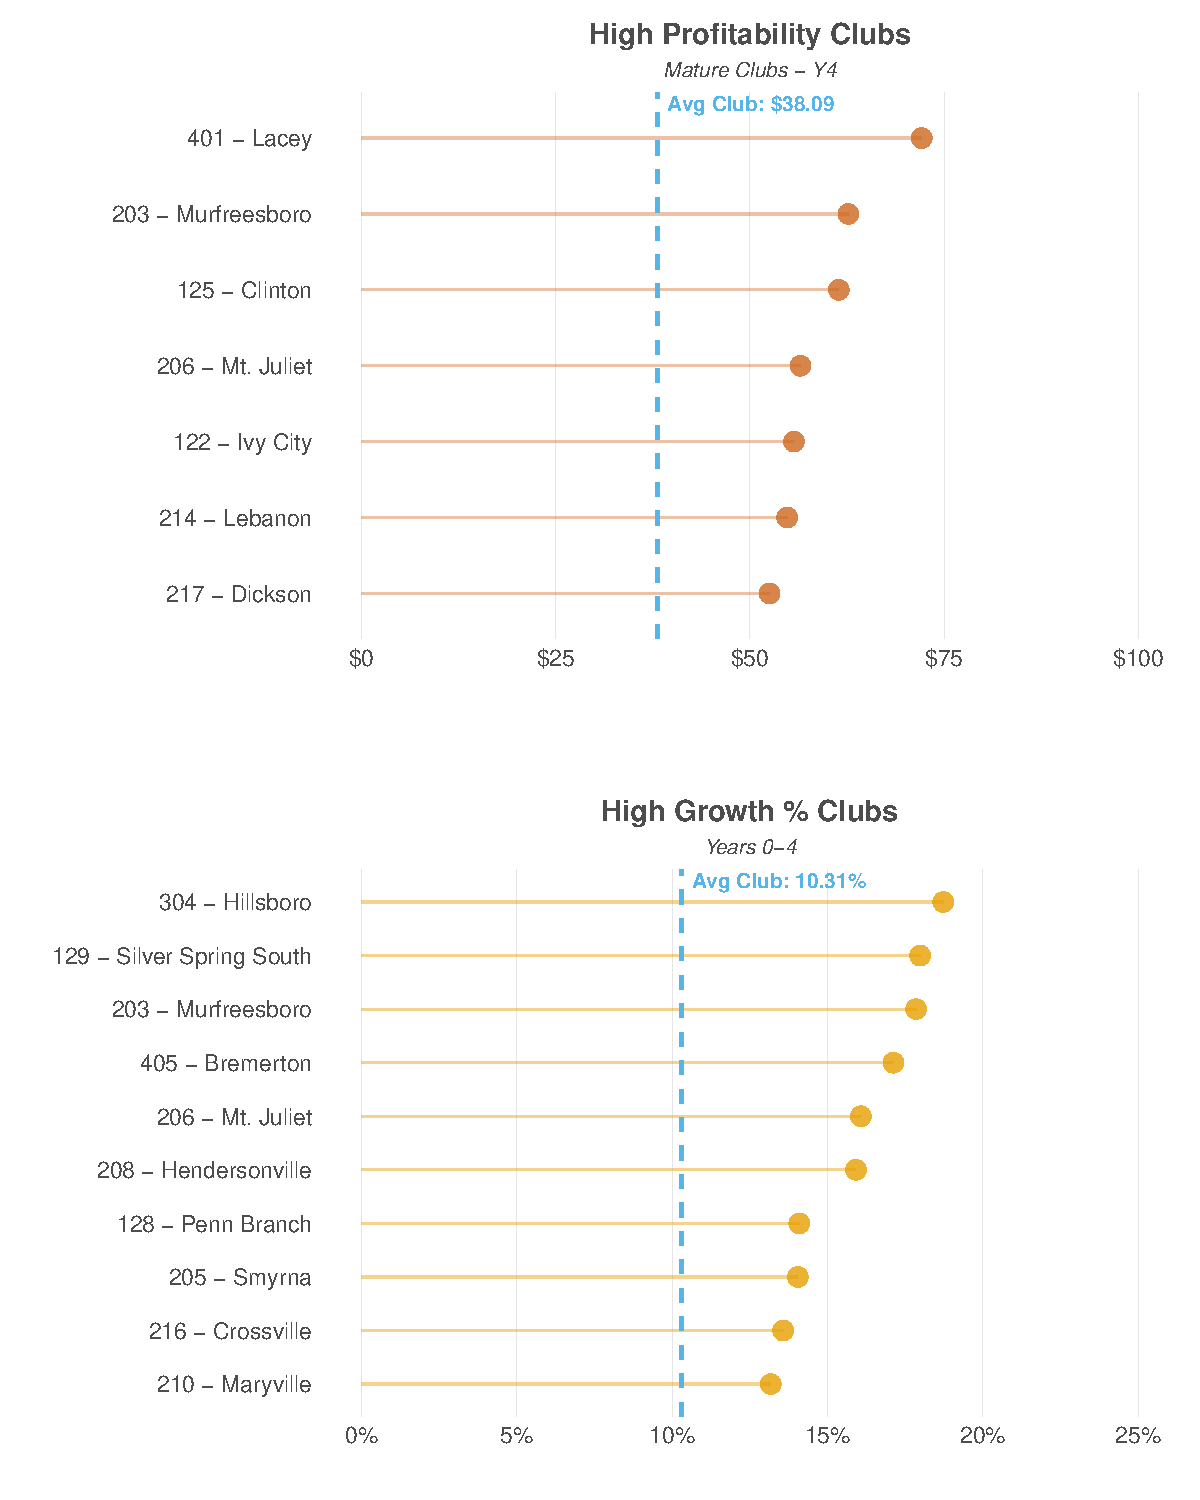
\includegraphics[keepaspectratio]{fit_report_profit_files/figure-pdf/top-clubs-1.pdf}}

\subsection{Feature Importance After Running Statistical
Model}\label{feature-importance-after-running-statistical-model}

\emph{Chart: What are the most important factors driving profitability?}

\emph{Text: Size, female population and RentPSF are the top three
factors.}

\begin{Shaded}
\begin{Highlighting}[]
\CommentTok{\# Chart: Sucess Factors Behind Profitability}
\CommentTok{\# Create the plot}
\FunctionTok{ggplot}\NormalTok{(rf\_importance, }\FunctionTok{aes}\NormalTok{(}\AttributeTok{x =}\NormalTok{ Importance, }\AttributeTok{y =}\NormalTok{ Variable, }\AttributeTok{fill =}\NormalTok{ Importance)) }\SpecialCharTok{+}
  \FunctionTok{geom\_col}\NormalTok{(}\AttributeTok{width =} \FloatTok{0.7}\NormalTok{, }\AttributeTok{alpha =} \FloatTok{0.9}\NormalTok{) }\SpecialCharTok{+}
  \FunctionTok{scale\_fill\_gradient}\NormalTok{(}
    \AttributeTok{low =} \StringTok{"\#0077bb"}\NormalTok{,}
    \AttributeTok{high =} \StringTok{"\#ee7733"}\NormalTok{,}
    \AttributeTok{name =} \StringTok{"Importance Score"}
\NormalTok{  ) }\SpecialCharTok{+}
  \FunctionTok{scale\_x\_continuous}\NormalTok{(}
    \AttributeTok{labels =}\NormalTok{ comma,}
    \AttributeTok{name =} \StringTok{"Importance Score"}
\NormalTok{  ) }\SpecialCharTok{+}
  \FunctionTok{labs}\NormalTok{(}
    \AttributeTok{title =} \StringTok{"Random Forest Feature Importance"}\NormalTok{,}
    \AttributeTok{subtitle =} \StringTok{"Top 20 Features by Mean Decrease in Gini"}\NormalTok{,}
    \AttributeTok{x =} \ConstantTok{NULL}\NormalTok{,}
    \AttributeTok{y =} \ConstantTok{NULL}
\NormalTok{  ) }\SpecialCharTok{+}
  \FunctionTok{theme\_minimal}\NormalTok{() }\SpecialCharTok{+}
  \FunctionTok{theme}\NormalTok{(}
    \AttributeTok{plot.title =} \FunctionTok{element\_text}\NormalTok{(}\AttributeTok{hjust =} \FloatTok{0.5}\NormalTok{, }\AttributeTok{face =} \StringTok{"bold"}\NormalTok{, }\AttributeTok{size =} \DecValTok{14}\NormalTok{),}
    \AttributeTok{plot.subtitle =} \FunctionTok{element\_text}\NormalTok{(}\AttributeTok{hjust =} \FloatTok{0.5}\NormalTok{, }\AttributeTok{size =} \DecValTok{10}\NormalTok{),}
    \AttributeTok{axis.text.y =} \FunctionTok{element\_text}\NormalTok{(}\AttributeTok{size =} \DecValTok{9}\NormalTok{, }\AttributeTok{color =} \StringTok{"black"}\NormalTok{),}
    \AttributeTok{legend.position =} \StringTok{"right"}\NormalTok{,}
    \AttributeTok{panel.grid.major.y =} \FunctionTok{element\_blank}\NormalTok{(),}
    \AttributeTok{panel.grid.minor =} \FunctionTok{element\_blank}\NormalTok{()}
\NormalTok{  )}
\end{Highlighting}
\end{Shaded}

\pandocbounded{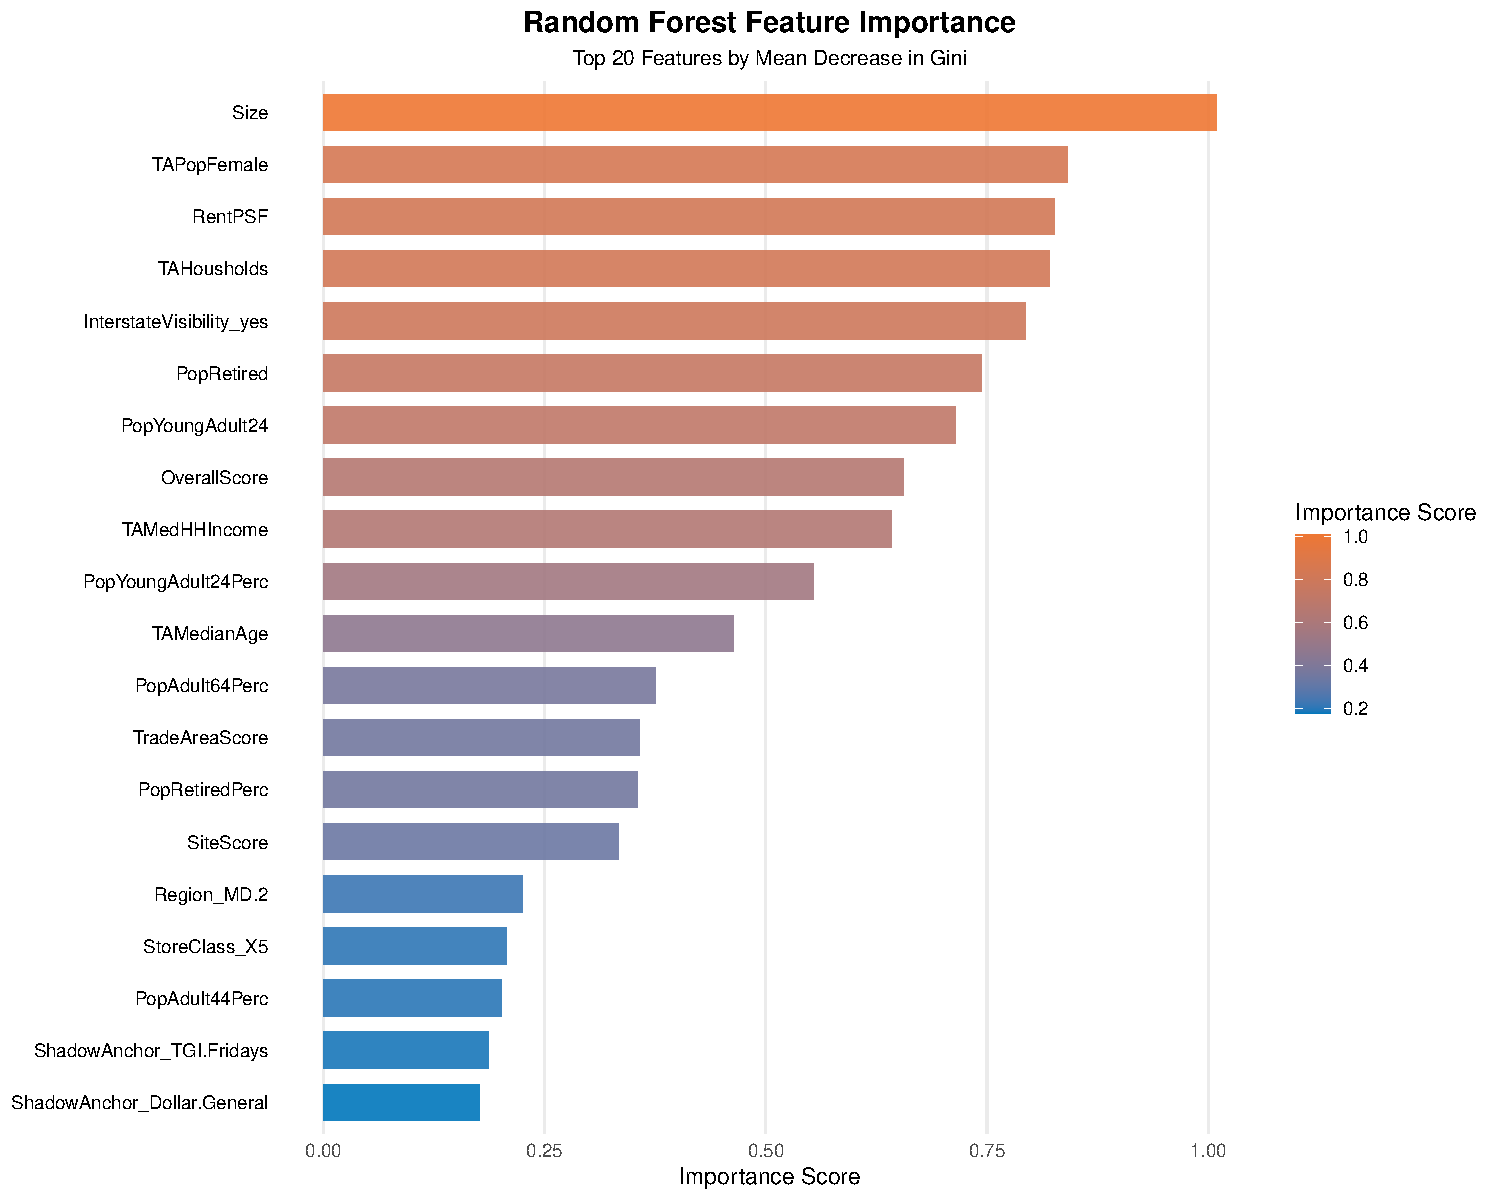
\includegraphics[keepaspectratio]{fit_report_profit_files/figure-pdf/feature-importance-1.pdf}}




\end{document}
